\begin{appendices}




\section{Likelihood of Merging Regions}
\label{sec:app_cost}
In a variety of computer vision applications such as region-based segmentation or region-based object proposals, the likelihood of merging two adjacent regions based on their appearance is considered~\cite{Uijlings:etal:IJCV13}. Let $\mu(A_i,A_j)$ reflect the similarity of merging regions $A_i$ and $A_j$ into $A_i \cup A_j$. Examples of such measures can be found in~\cite{Uijlings:etal:IJCV13,Xiao:Lu:etal:CVPR15,Bonev:Yuille:ECCV14} which are typically based on compatibility of intensity, color, texture, and size of regions. We adopt a similar measure as in {\bf Selective Search}~\cite{Uijlings:etal:IJCV13} which is based on texture and color histograms. Specifically, for each region we compute a $LAB$ histogram, $H_i$, which is a combination of three 1D histograms based on the $L$, $A$, and $B$ channels of the LAB color space. We also compute a histogram of textons, $T_i$, to capture texture. The pairwise similarity of these descriptors is measured using histogram intersection. The final similarity of two regions, $\mu(A_i,A_j)$, is then measured as a weighted linear combination of the similarity of the color and texture descriptors respectively, Equation~\ref{eq:sim}.

\begin{equation}
\begin{split}
\mu(A_i,A_j) &= \lambda\mu_{color}(A_i,A_j)+(1-\lambda)\mu_{texture}(A_i,A_j) \\
             &= \lambda\sum_k^M\min(H_i^k,H_j^k)+ (1-\lambda)\sum_k^M\min(T_i^k,T_j^k)
\end{split}
\label{eq:sim}
\end{equation}

\begin{figure*}[!ht]
\centering
\setlength{\tabcolsep}{2pt}
\begin{tabular}{cc}
{\footnotesize\textit{\textcolor{black}{a)}}}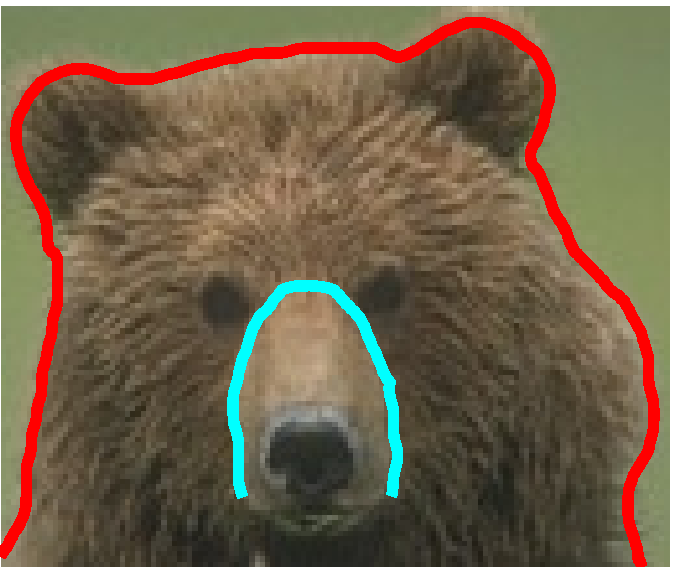
\includegraphics[width=0.11\textwidth]{figs/bear_l1.pdf}&\multirow{3}{*}[0.45in]{{\footnotesize\textit{\textcolor{black}{d)}}}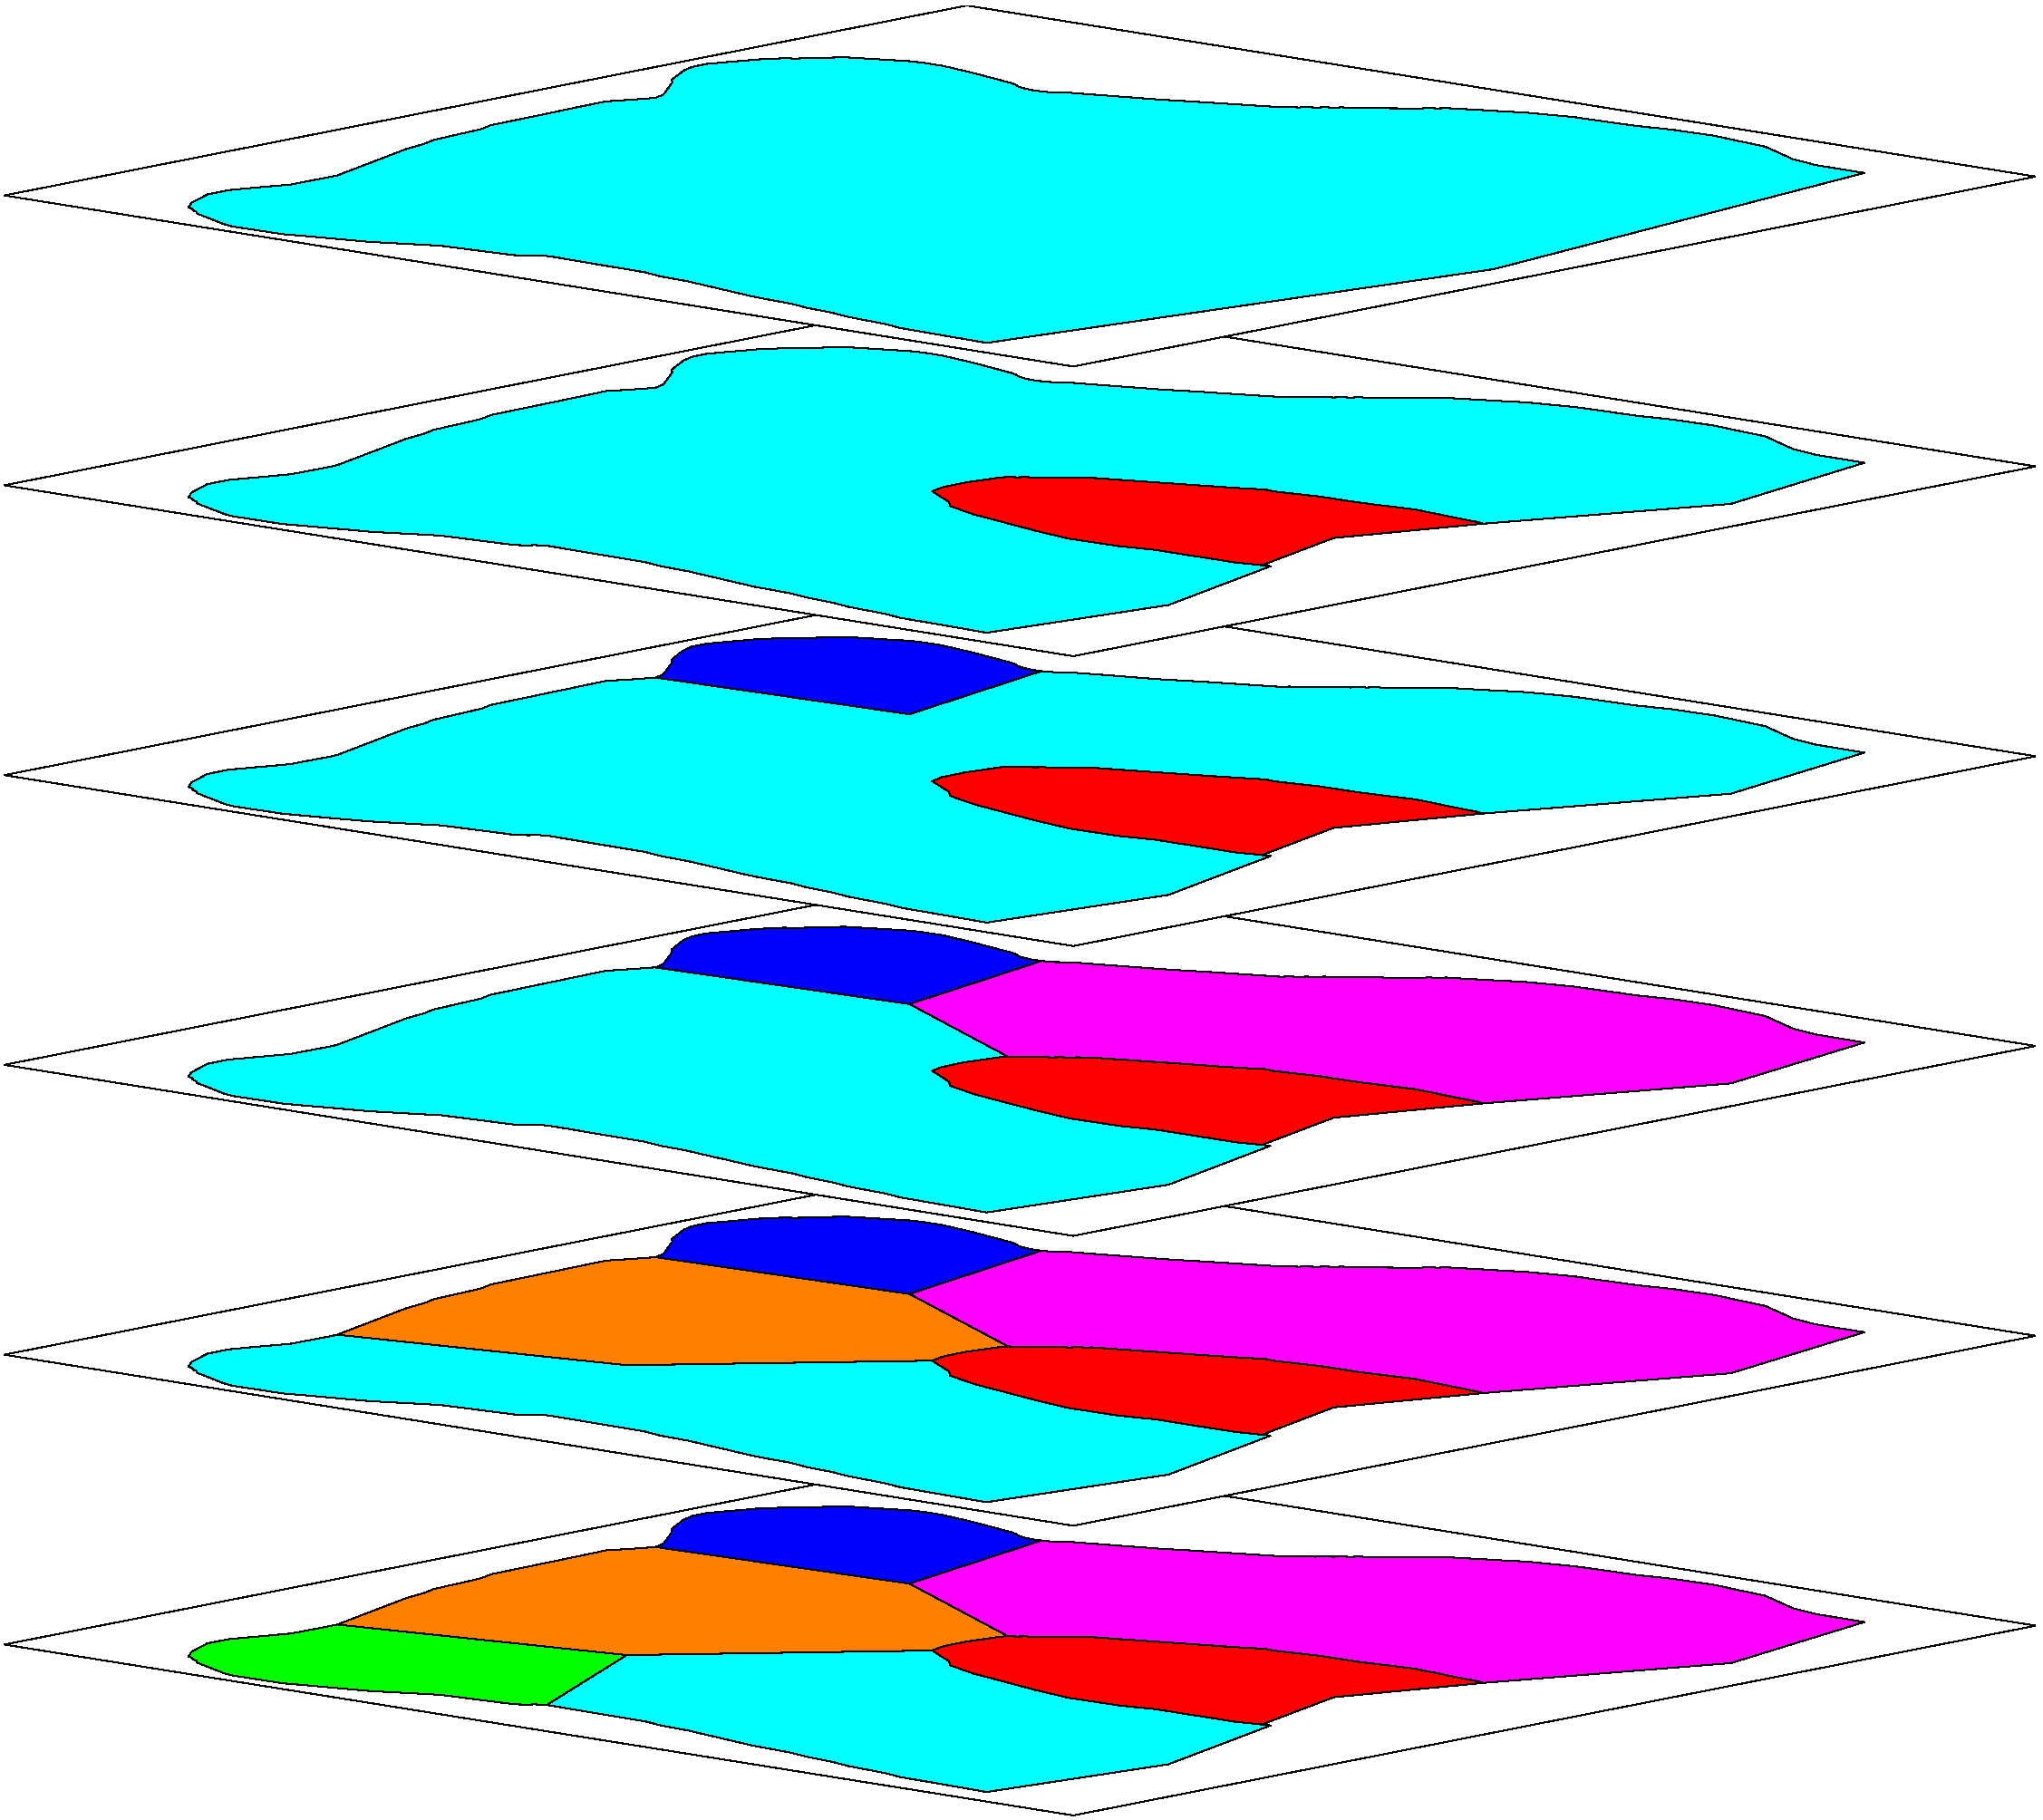
\includegraphics[width=0.3\textwidth]{figs/bear_l4.pdf}}\\
{\footnotesize\textit{\textcolor{black}{b)}}}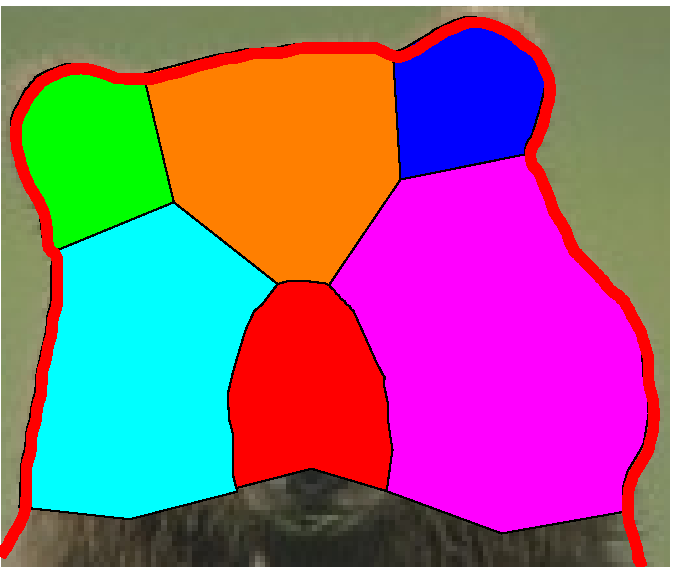
\includegraphics[width=0.11\textwidth]{figs/bear_l2.pdf}\\
{\footnotesize\textit{\textcolor{black}{c)}}}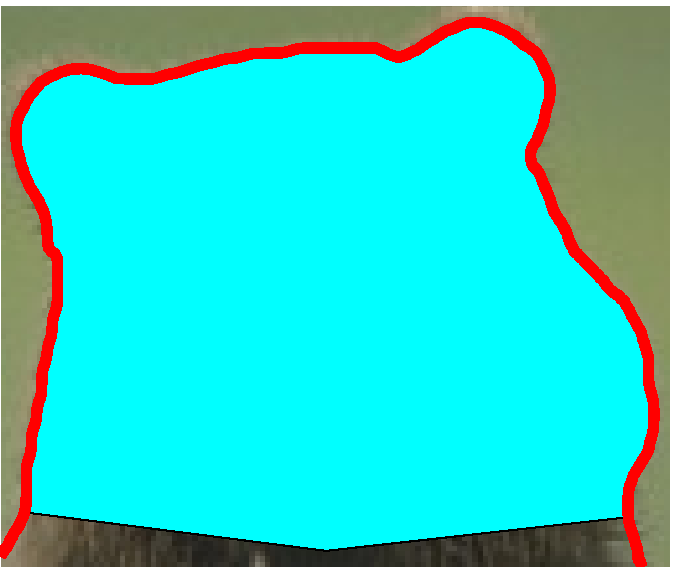
\includegraphics[width=0.11\textwidth]{figs/bear_l3.pdf}\\
\end{tabular}
\begin{tabular}{cc}
{\footnotesize\textit{\textcolor{black}{e)}}}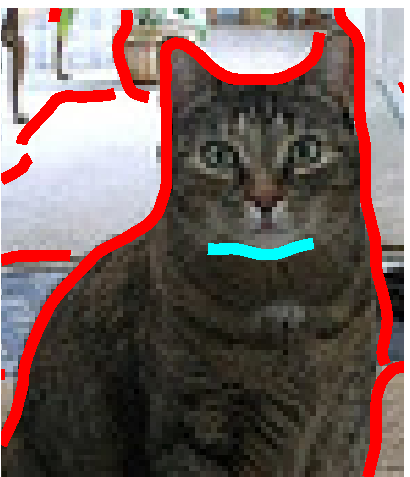
\includegraphics[height=0.09\textwidth]{figs/cat1.pdf}&\multirow{3}{*}[0.45in]{{\footnotesize\textit{\textcolor{black}{h)}}}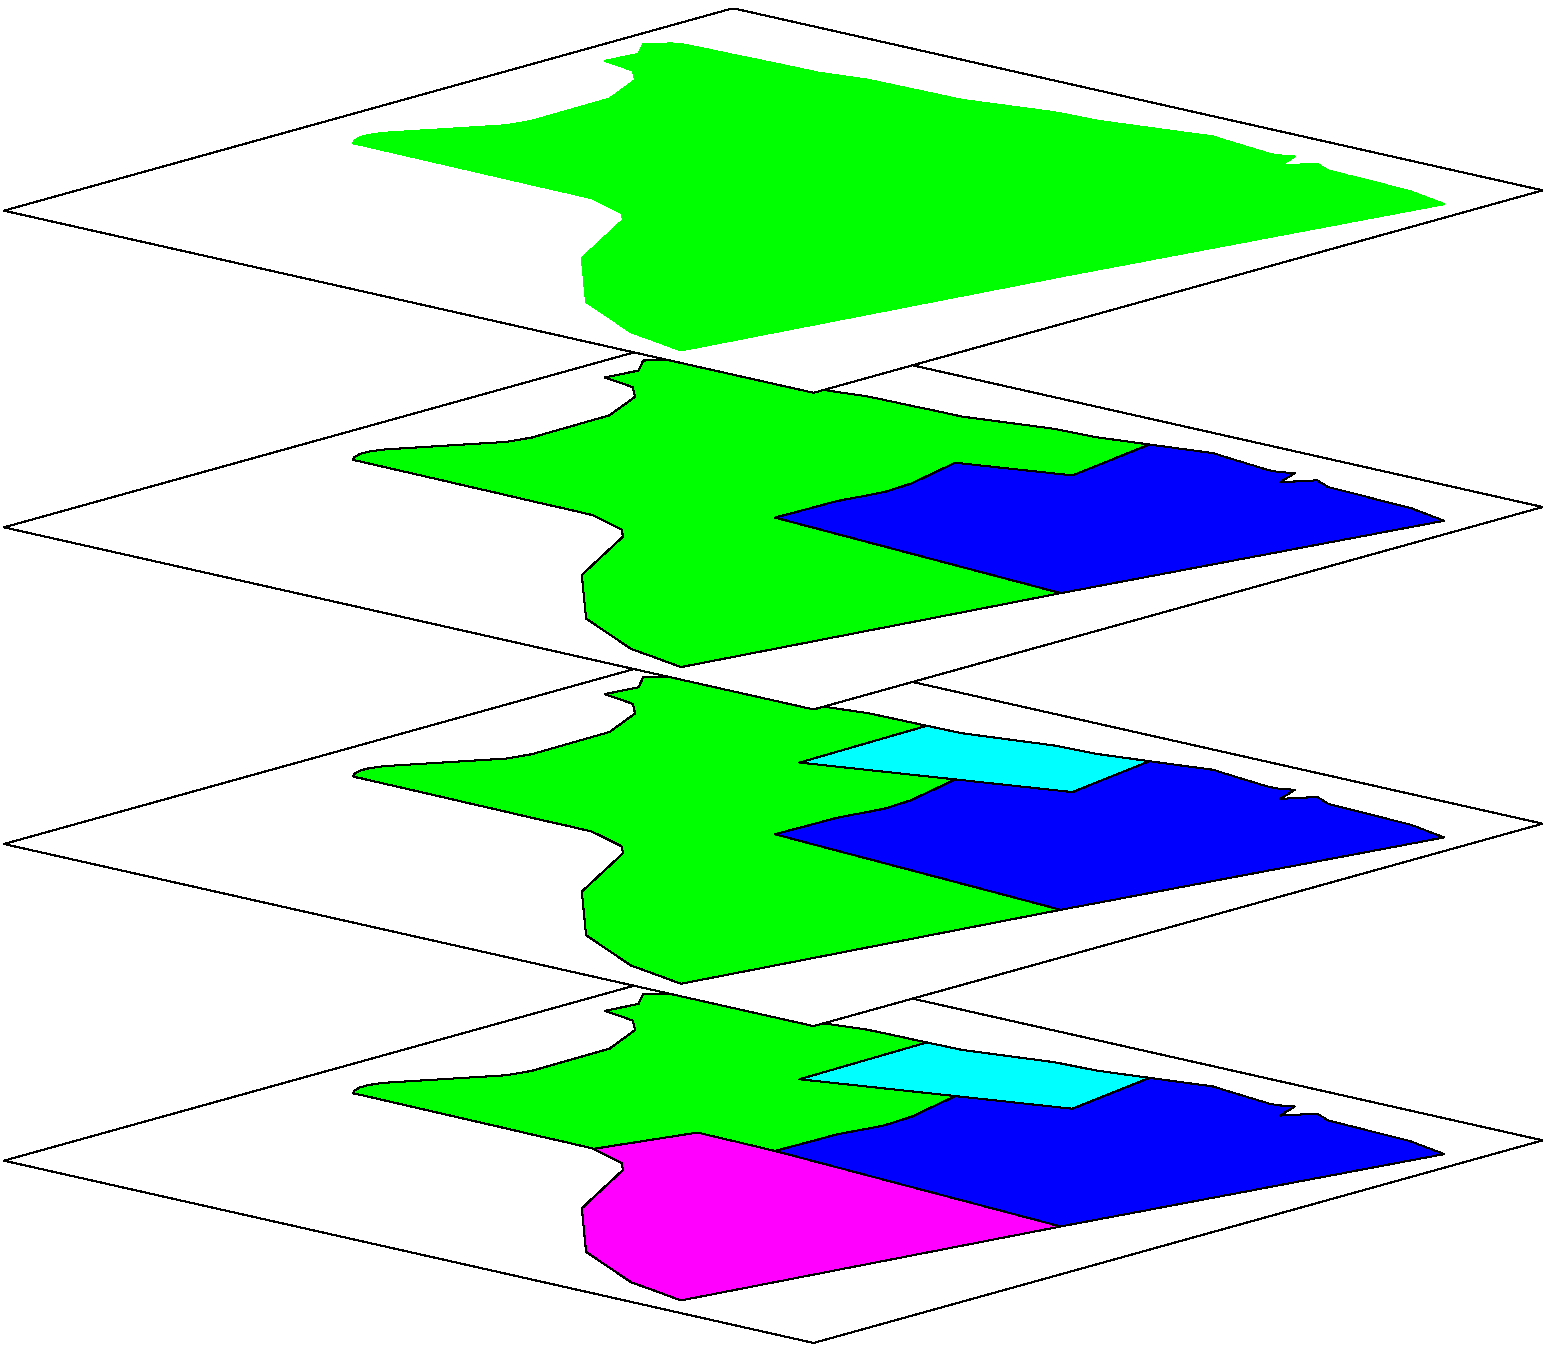
\includegraphics[width=0.3\textwidth]{figs/cat4.pdf}}\\
{\footnotesize\textit{\textcolor{black}{f)}}}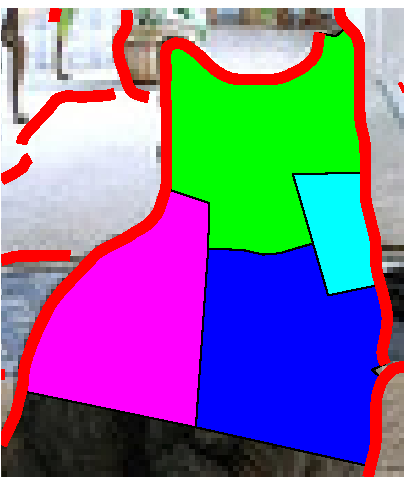
\includegraphics[height=0.09\textwidth]{figs/cat2.pdf}\\
{\footnotesize\textit{\textcolor{black}{g)}}}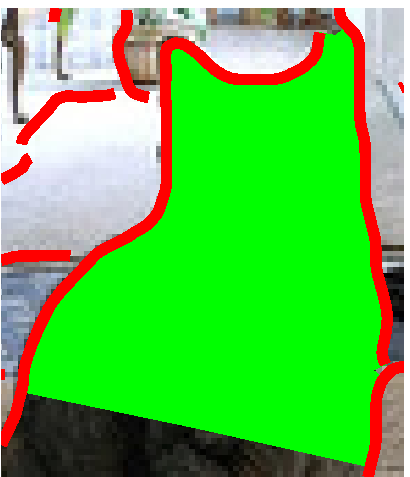
\includegraphics[height=0.09\textwidth]{figs/cat3.pdf}\\
\end{tabular}
\caption{a,e) We show two examples where we are considering the removal of the \textcolor{cyan}{cyan} curve surrounded by the \textcolor{red}{red} silhouette curve. For clarity we have removed the shock graph. b,f) If we look at the initial set of fragmented medial visual fragments we see that the effect of removing this contour causes all regions to merge in both cases. d,h) The merging of $N$ regions to 1 can be expressed as a region hierarchy.}
\label{fig:loop_cost2}
\end{figure*}

The likelihood can be extended to that of merging $N$ regions, $\mu(A_1,A_2,...,A_N)$. The merge can be defined as an iterative grouping of pairs of regions until only one region remains, Figure~\ref{fig:loop_cost2}. Its likelihood is then the most likely path over all possible combinations of pairs. However, a greedy approximation is to only consider pairs composed of neighboring regions. At each iteration the two most similar neighboring regions that maximize Equation~\ref{eq:sim} are merged and the process is repeated. This avoids the costly consideration of all paths. The final likelihood, $\mu(A_1,A_2,...,A_N)$,  is therefore the product of the individual probabilities, Equation~\ref{eq:sim}, of all pairwise merges. 


%% \begin{equation}
%% \mu(A_1,A_2,...,A_N)=\prod_{i=0}^{N-2}\argmax_{(i,j)=\binom{N-i}{2}}\mu(A_i,A_j)
%% \label{eq:loop_prob}
%% \end{equation}

%% \noindent
%% {\bf Normalization: } The final likelihood of merging $N$ regions into one is based on the product of successive pairwise merges. The probability though is not invariant to the initial number of regions, $N$. The likelihood will in general be larger the less fragments that are initially present. To deal with this we observe that the major decision when 

%% \chapter{Computational Complexity}
%% \label{sec:cc}
%% In what follows we discuss the computational complexity of our object proposal algorithm, Chapter~\ref{chapter:ops}. Given that it is difficult to come up with a closed form expression for the behavior of our system we empirically observe the performance as a function of the number of contours. We measure complexity as the size (nodes) of the containment graph while varying the number of input contours to our system. Figure~\ref{fig:cgraph_growth} shows the growth of the containment graph across various images for various number of contours. Observe that irrespective of the number of contours the search space does not grow indefinitely but reaches a peak and then starts decreasing. Finally, over many images and many contour settings we fit a curve which gives an estimate of the size of the containment graph for any number of contours, Figure~\ref{fig:gg_growth}. Overall, the rate of growth of the curve limits the number of contours we can work with. 

%% \begin{figure*}[ht]
%% \centering
%% \setlength{\tabcolsep}{2pt}
%% \begin{tabular}{|cc|cc|}
%% \hline
%% 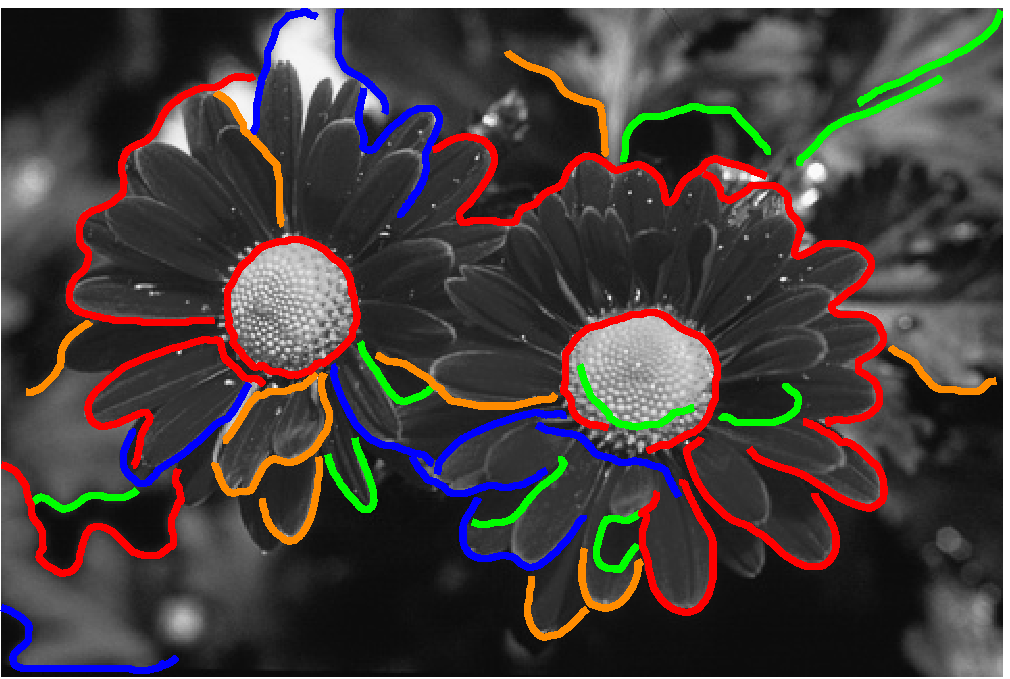
\includegraphics[width=0.24\linewidth]{figs/124084_cons_stats.pdf} &
%% 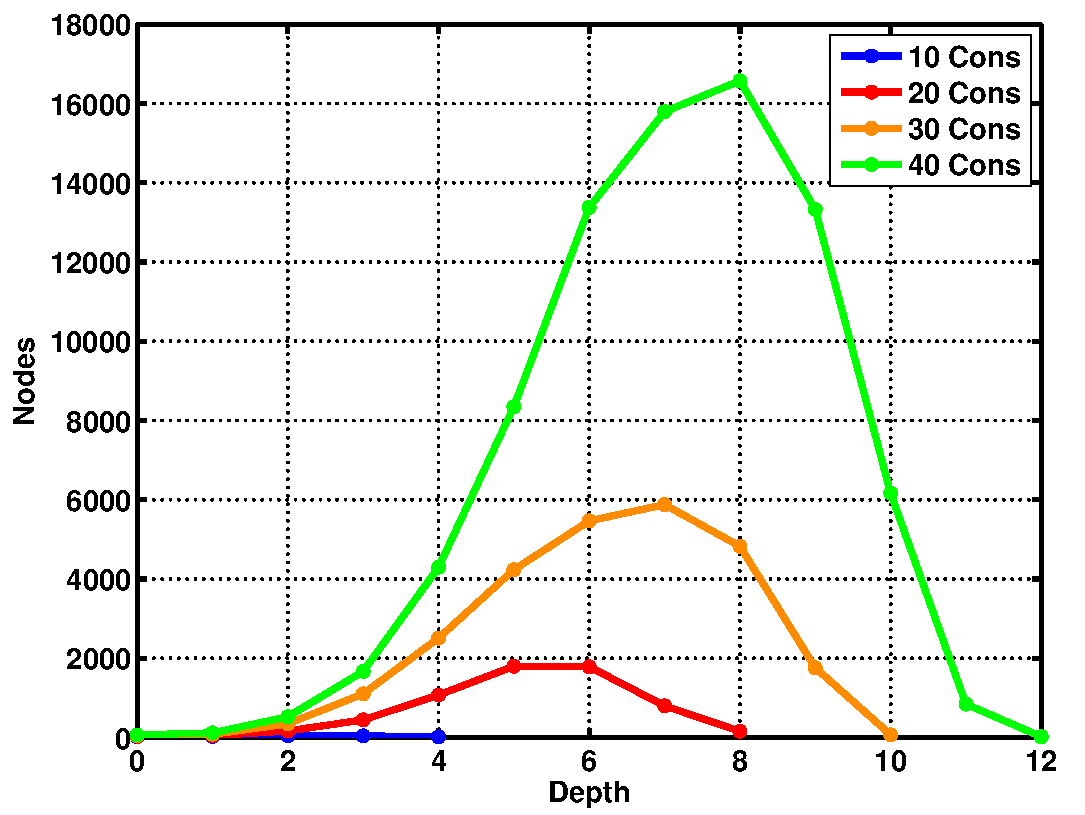
\includegraphics[width=0.24\linewidth]{figs/124084_stats.pdf} &
%% 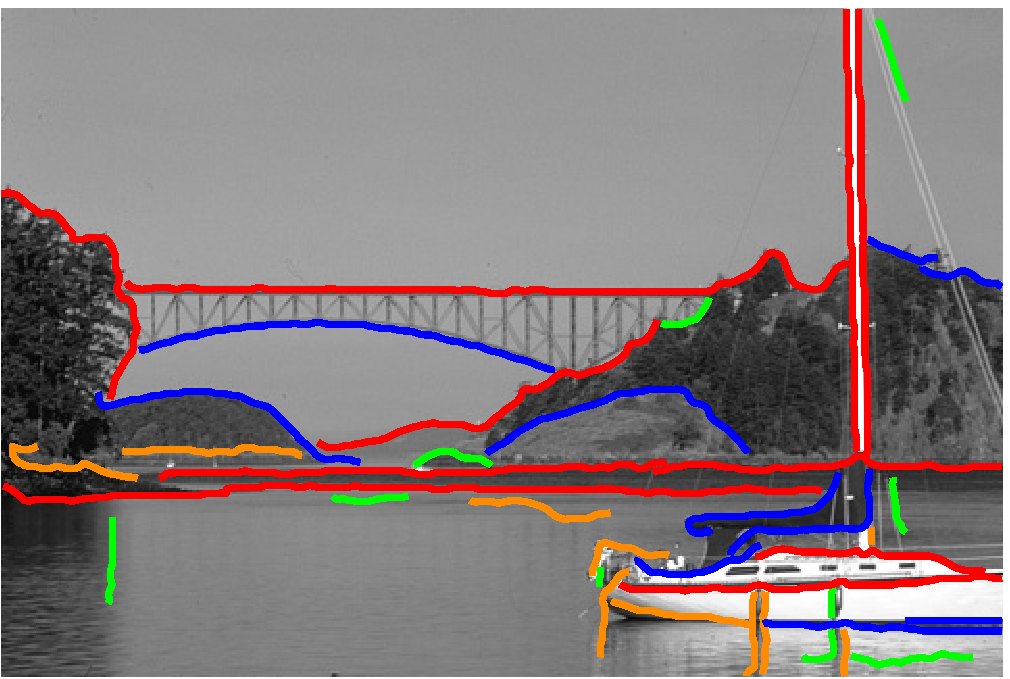
\includegraphics[width=0.24\linewidth]{figs/22090_cons_stats.pdf} &
%% 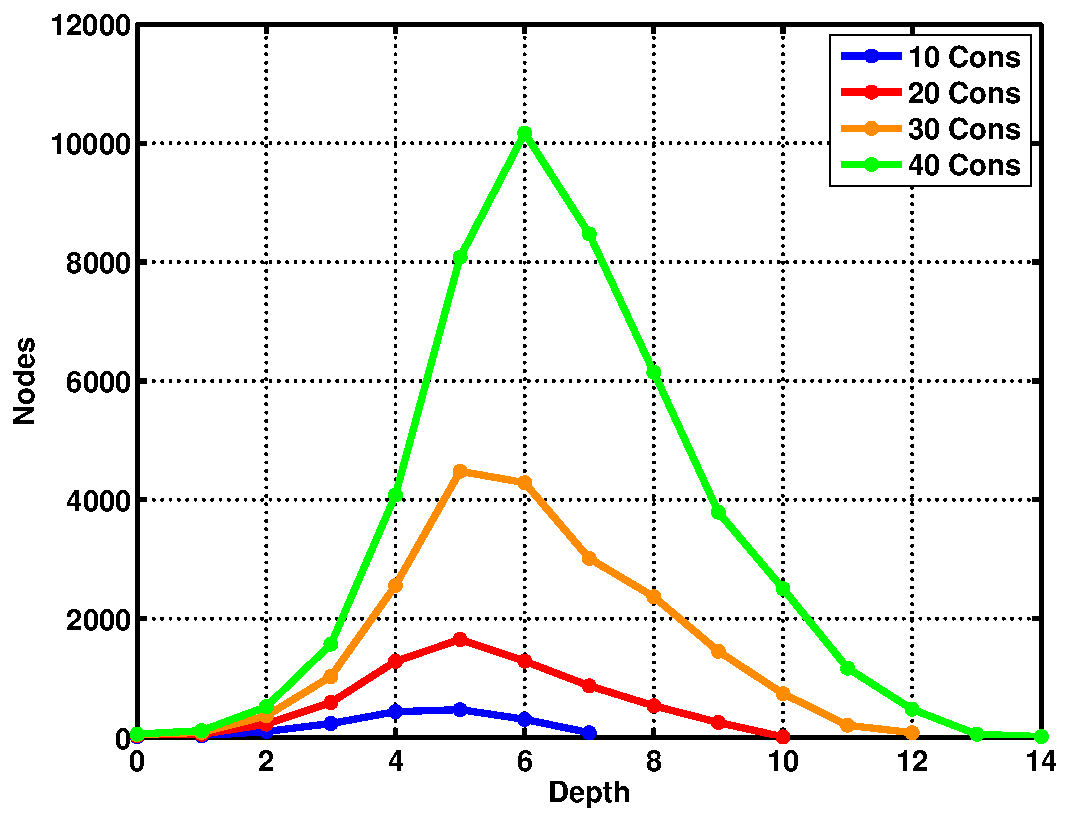
\includegraphics[width=0.24\linewidth]{figs/22090_stats.pdf} \\
%% \hline
%% 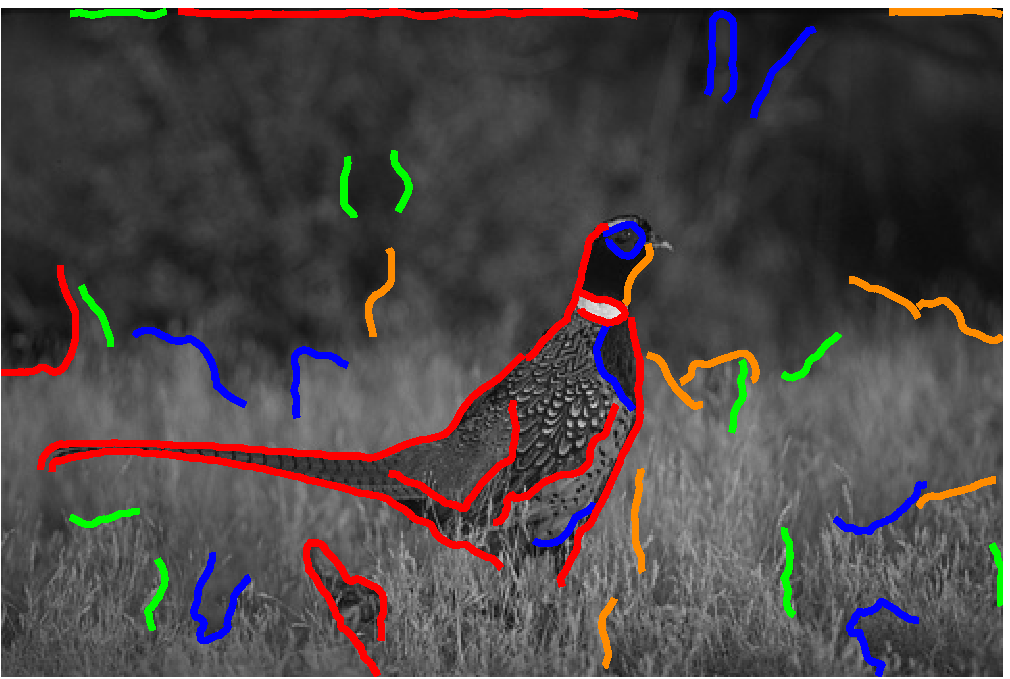
\includegraphics[width=0.24\linewidth]{figs/43074_cons_stats.pdf} &
%% 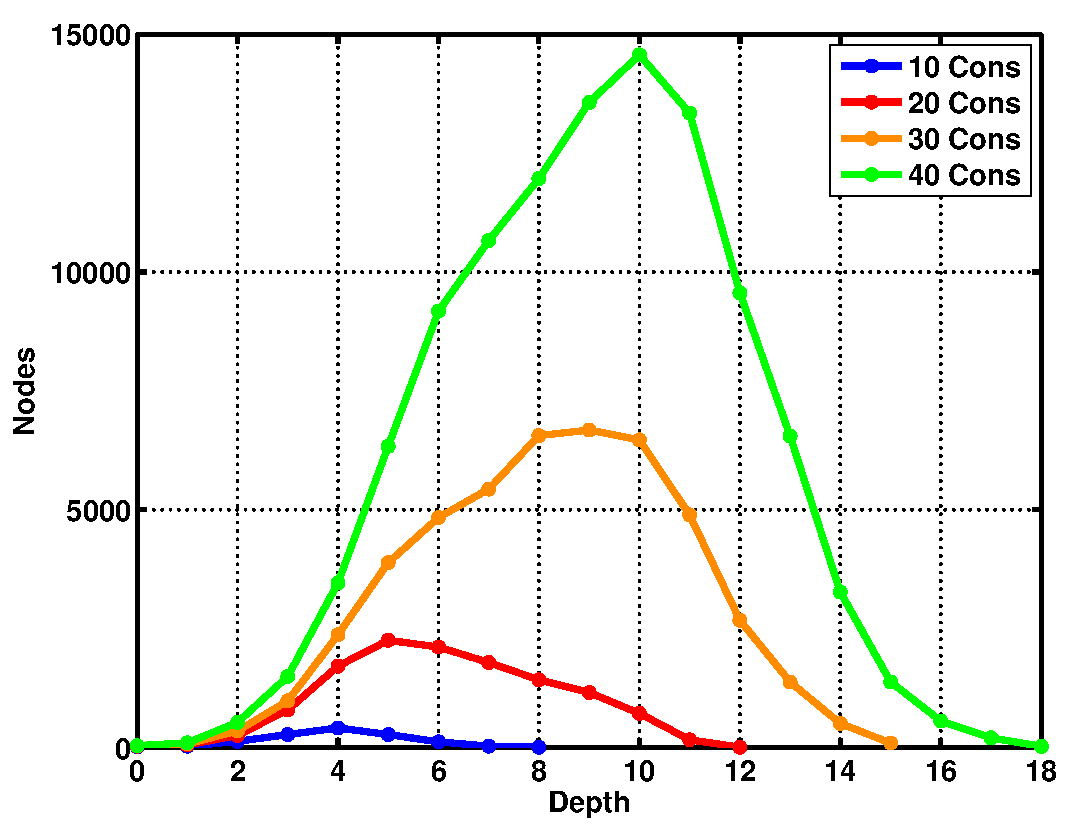
\includegraphics[width=0.24\linewidth]{figs/43074_stats.pdf} &
%% 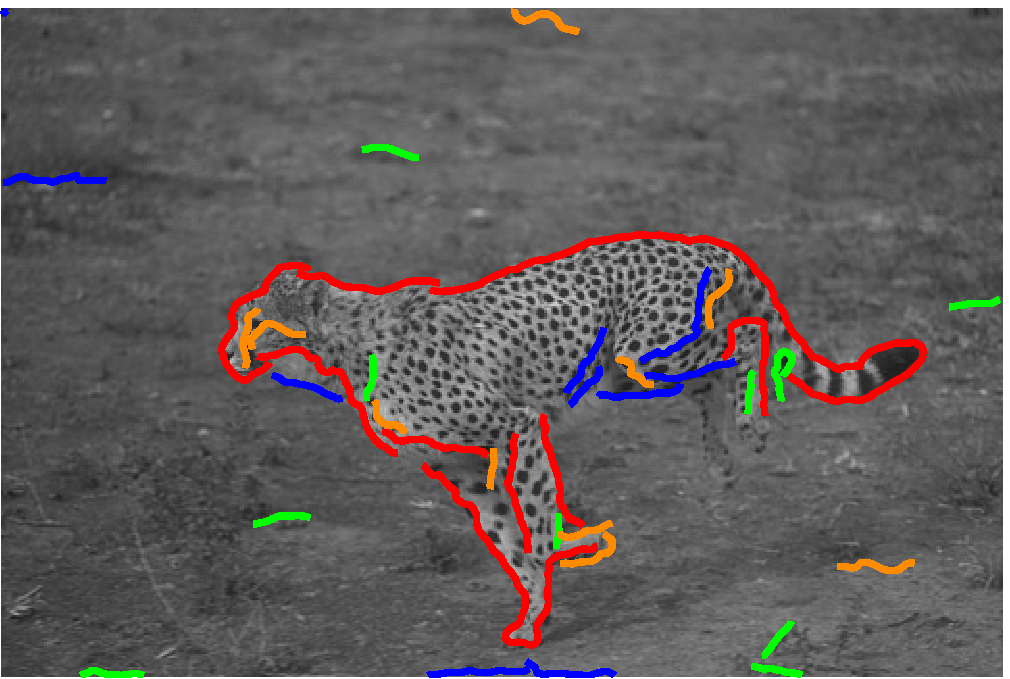
\includegraphics[width=0.24\linewidth]{figs/134008_cons_stats.pdf} &
%% 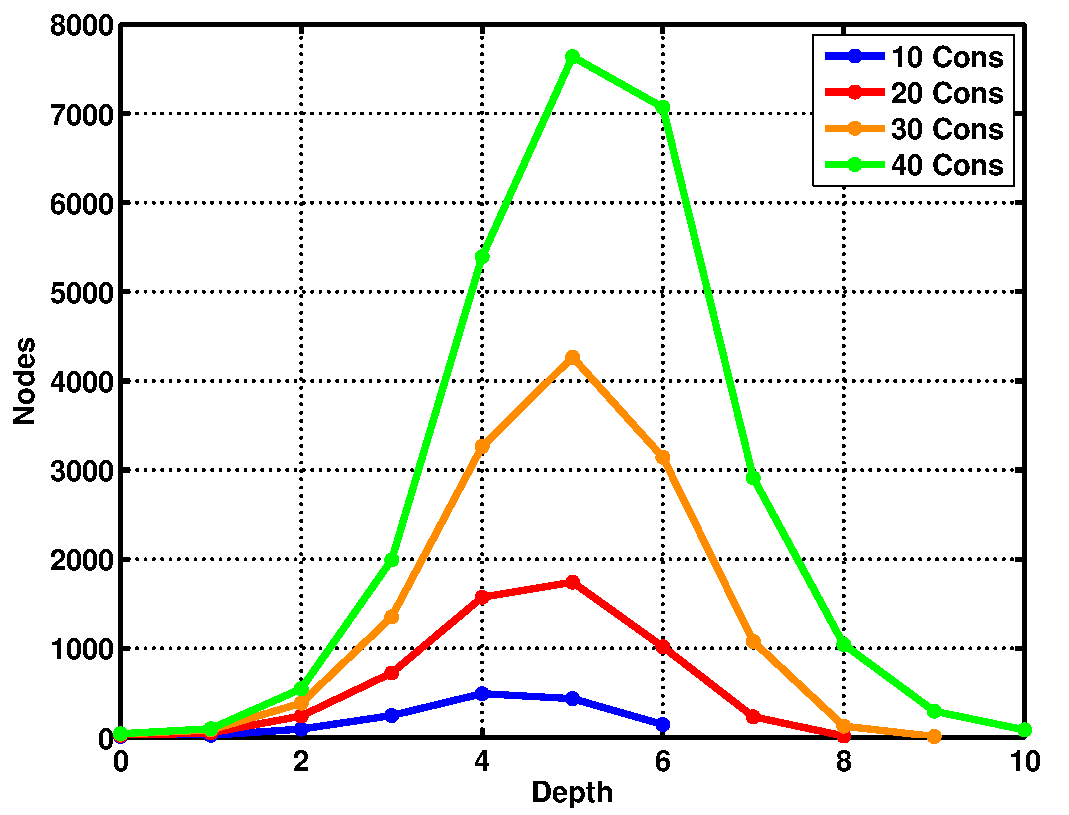
\includegraphics[width=0.24\linewidth]{figs/134008_stats.pdf} \\
%% \hline
%% 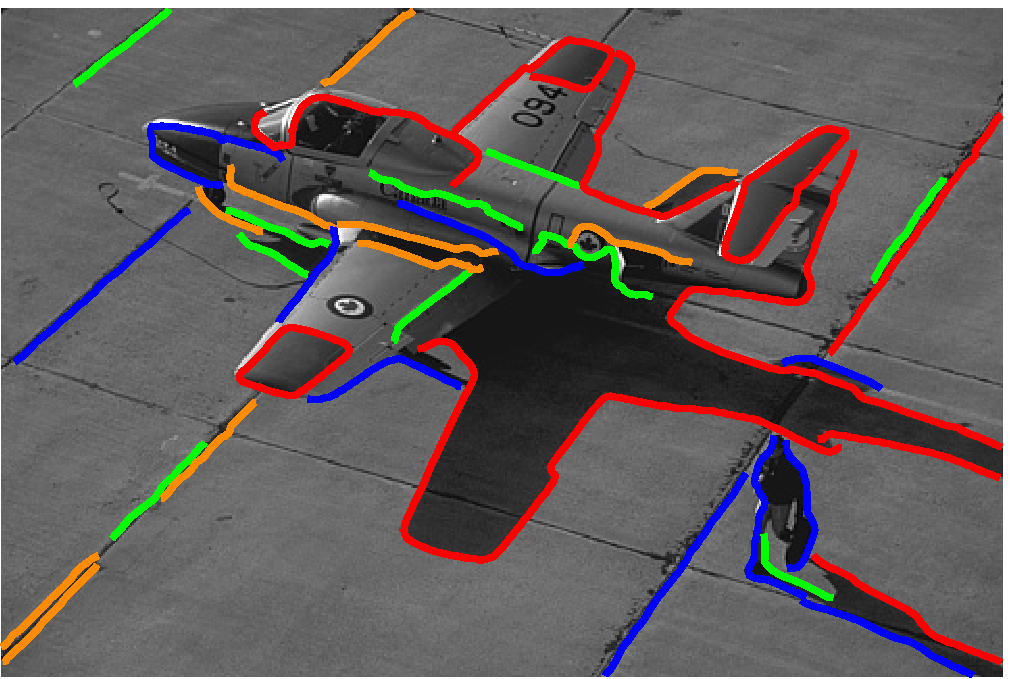
\includegraphics[width=0.24\linewidth]{figs/37073_cons_stats.pdf} &
%% 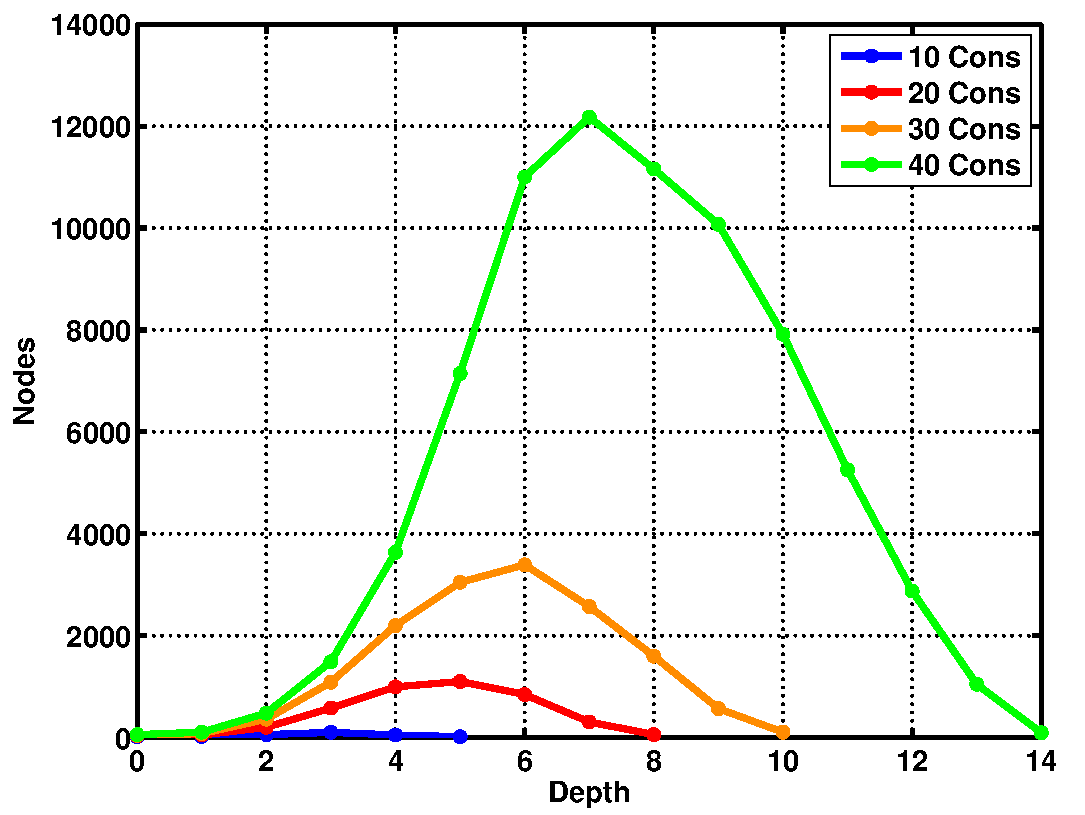
\includegraphics[width=0.24\linewidth]{figs/37073_stats.pdf} &
%% 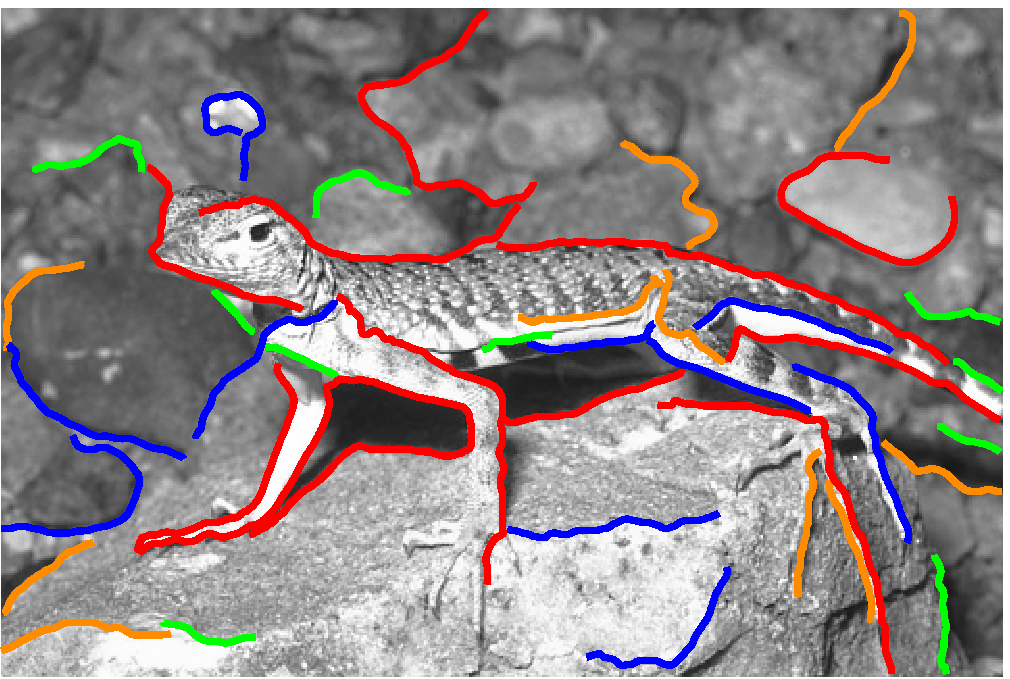
\includegraphics[width=0.24\linewidth]{figs/87046_cons_stats.pdf} &
%% 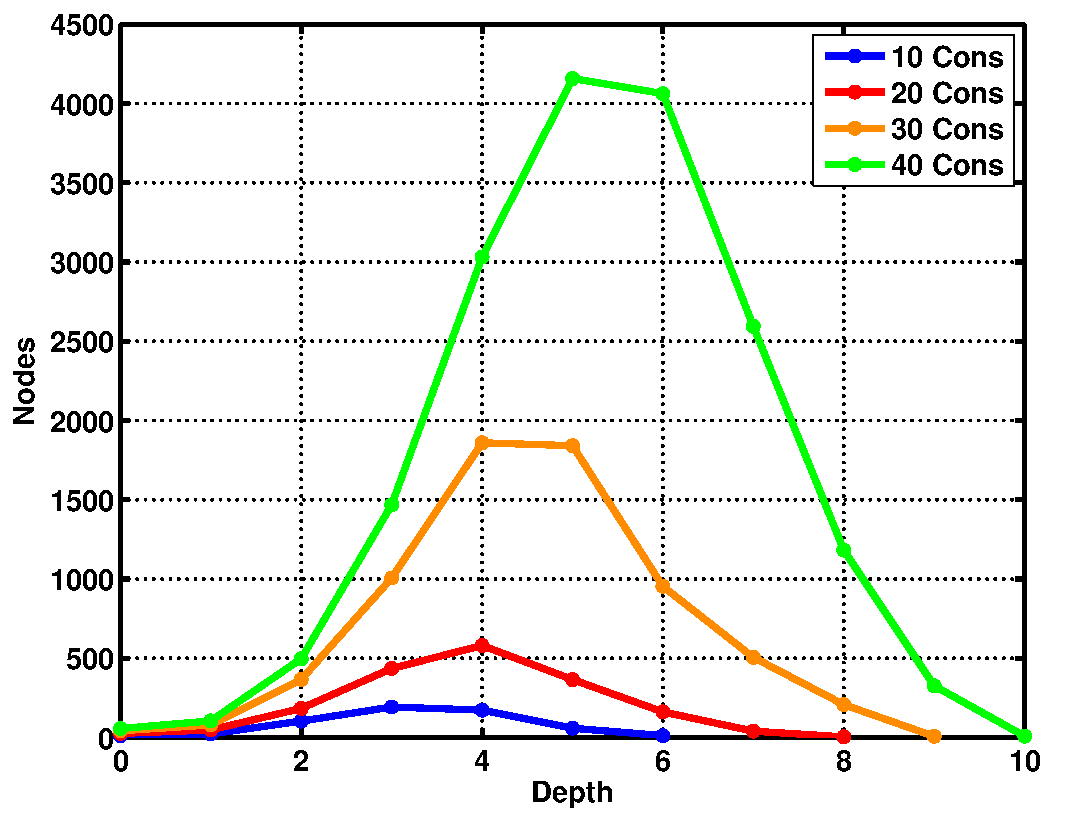
\includegraphics[width=0.24\linewidth]{figs/87046_stats.pdf} \\
%% \hline
%% 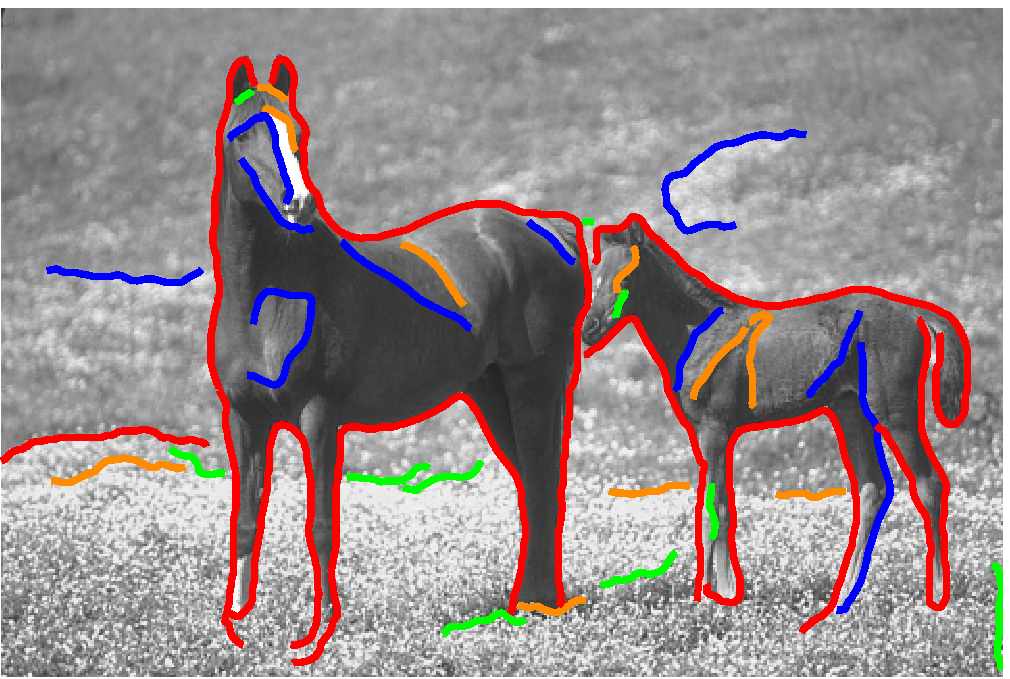
\includegraphics[width=0.24\linewidth]{figs/113016_cons_stats.pdf} &
%% 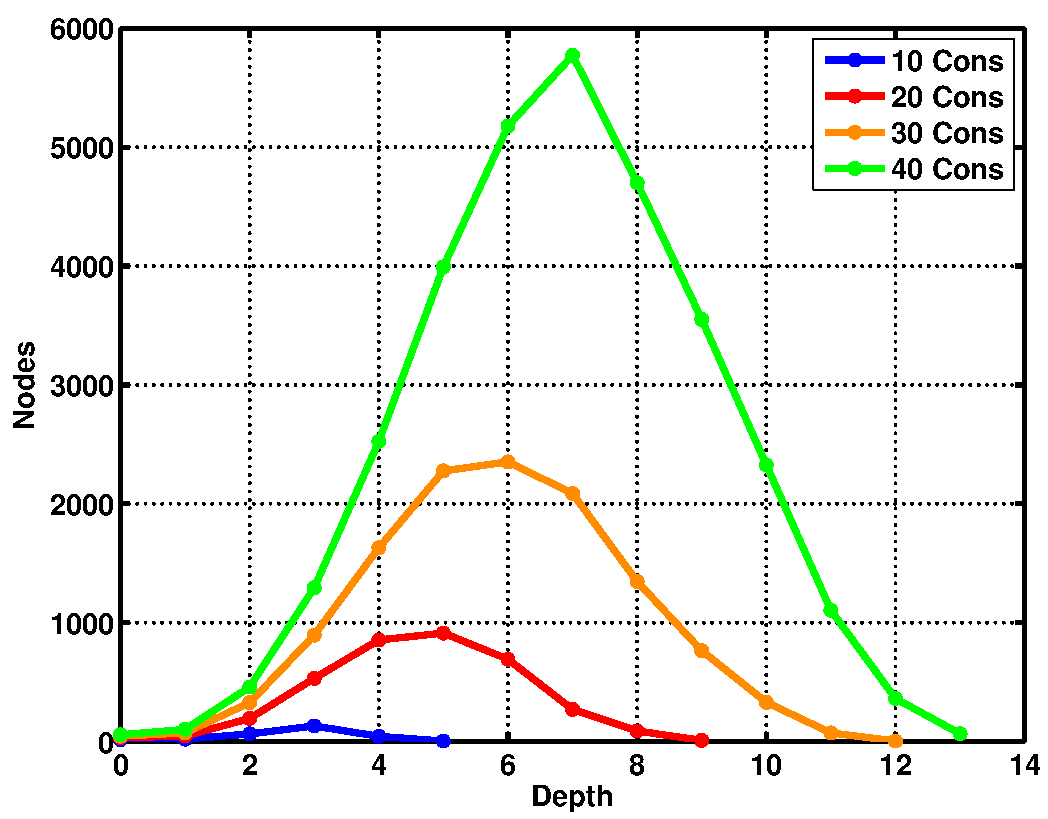
\includegraphics[width=0.24\linewidth]{figs/113016_stats.pdf} &
%% 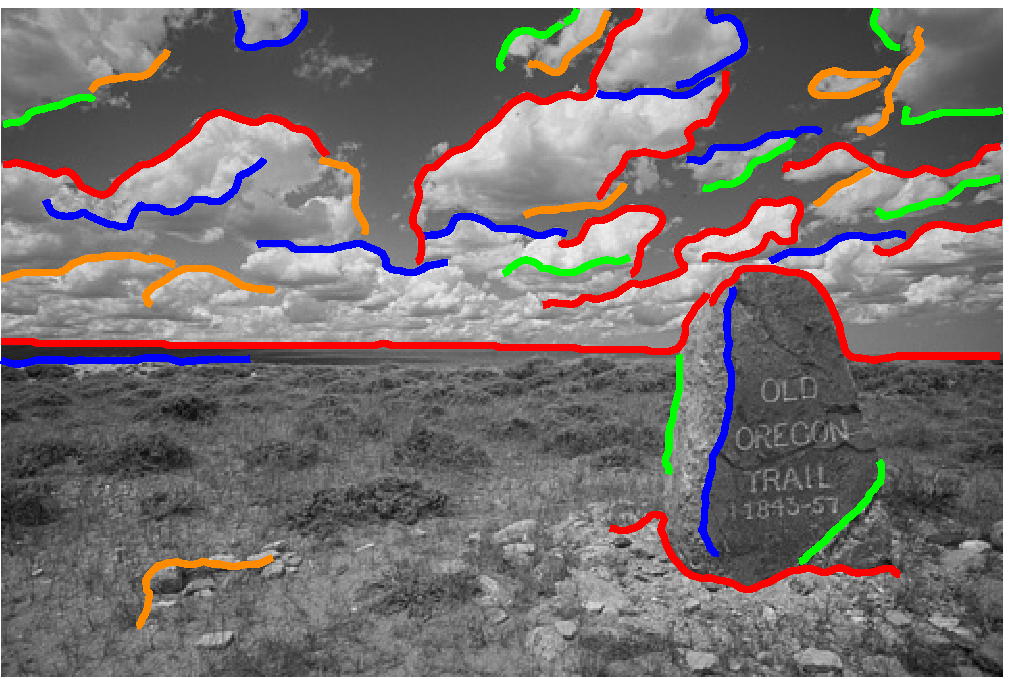
\includegraphics[width=0.24\linewidth]{figs/216066_cons_stats.pdf} &
%% 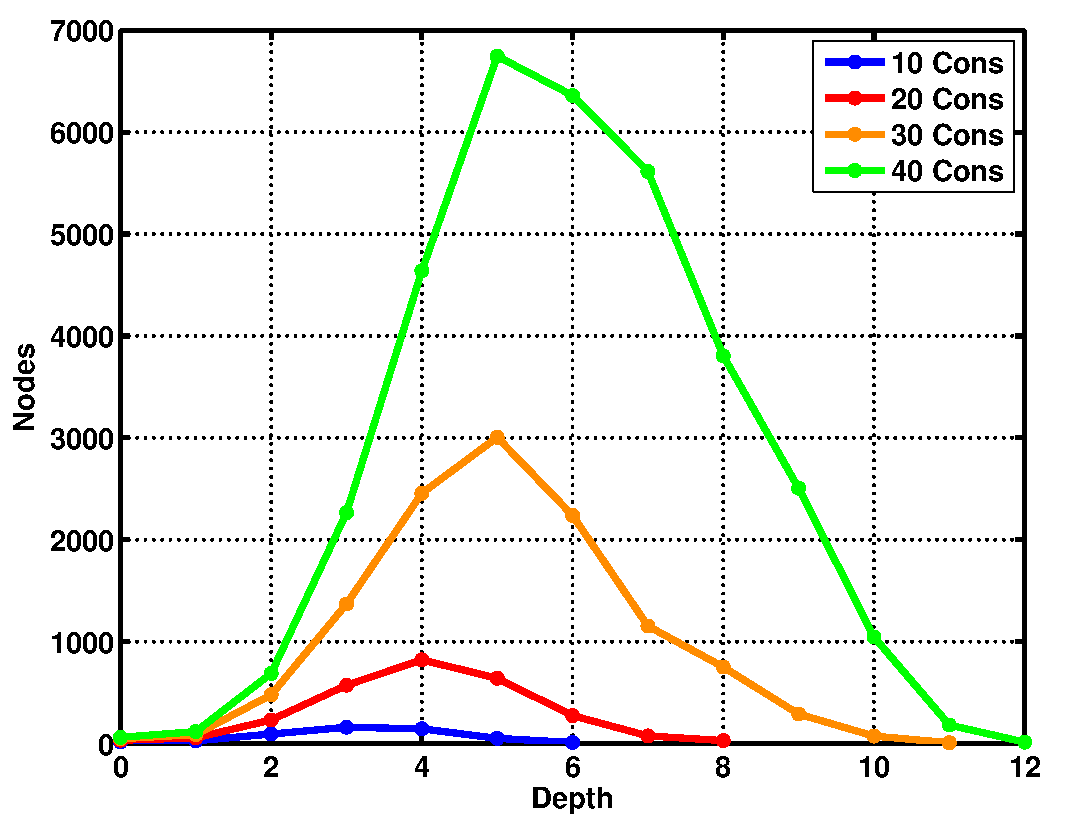
\includegraphics[width=0.24\linewidth]{figs/216066_stats.pdf} \\
%% \hline
%% \end{tabular}
%% \caption{The relationship between the number of nodes in our search space versus the number of contours in an image.  Each image is overlaid with 40 contours (green), 30 contours (orange), 20 contours (red), and 10 contours (blue). Observe how the growth of the search space irrespective of the number of contours reaches a peak and then starts decreasing. This reflects that the various groupings options have been exhausted and no new transform or transform sequences have developed. We observe that this peak shifts as the number of contours are increased.}
%% \label{fig:cgraph_growth}
%% \end{figure*}

%% \begin{figure*}[!ht]
%% \centering
%% 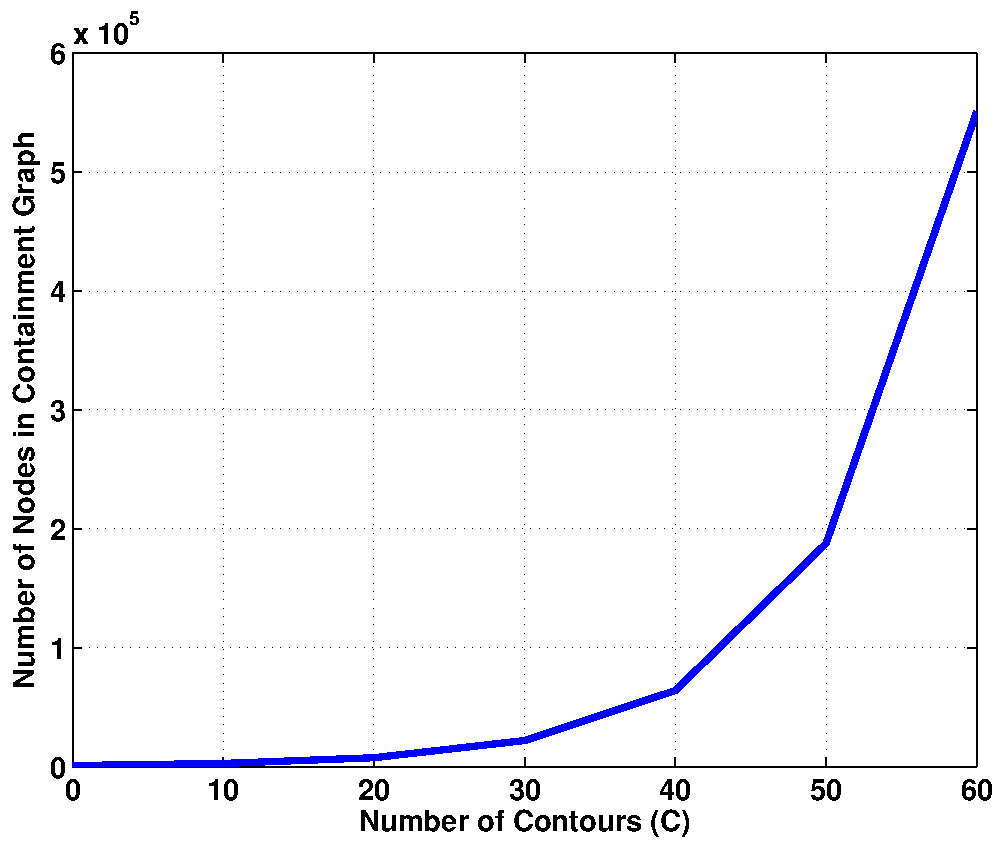
\includegraphics[width=0.35\linewidth]{figs/cgraph_growth.pdf}
%% %% {\footnotesize\textit{b}}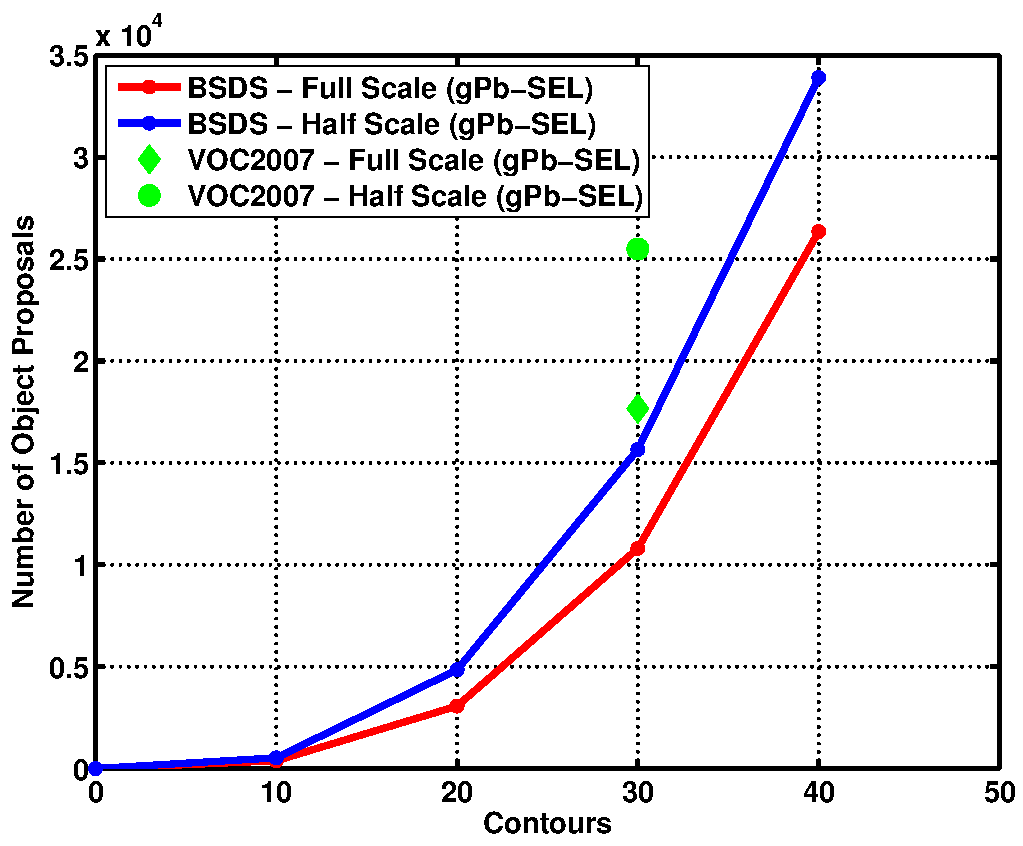
\includegraphics[width=0.47\linewidth]{figs/ops_vs_contours.pdf}
%% %% {\footnotesize\textit{d}}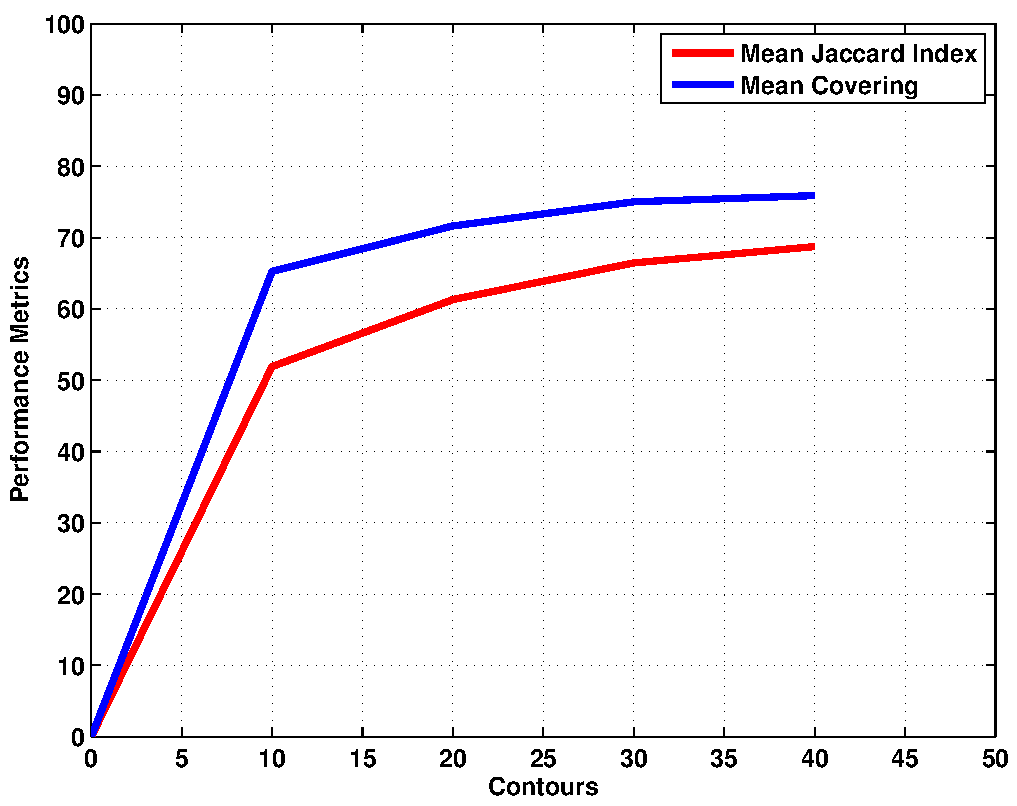
\includegraphics[width=0.47\linewidth]{figs/bsds_performance_vs_contours.pdf}
%% %% {\footnotesize\textit{e}}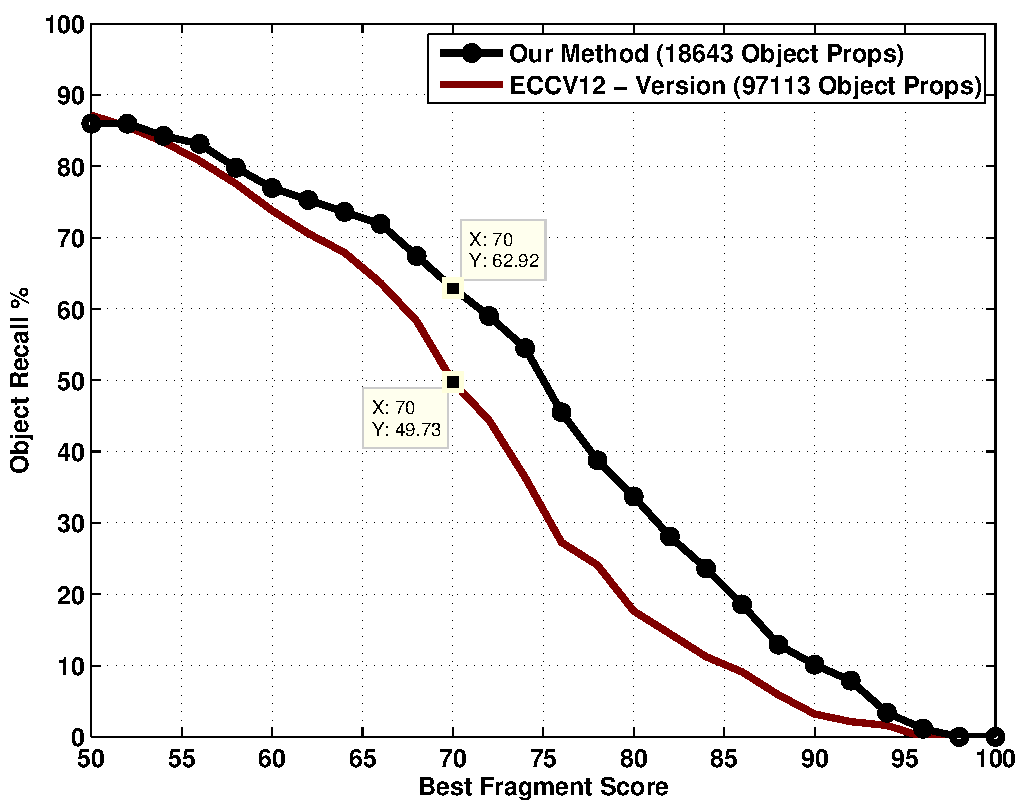
\includegraphics[width=0.47\linewidth]{figs/current_vs_eccv12.pdf}
%% \caption{We observe an exponential relationship between the number of contours and the size of the containment graph. }
%% \label{fig:gg_growth}
%% \end{figure*}

\section{Local Shock Computation}
\label{sec:lsc}

The computation of a shock graph from a static contour map is well established in the medial axis community.  What has received considerably less attention in the medial axis community is the case where the contour set is dynamic. A naive approach to this problem would be to re-compute the shock graph for every change (insertion or deletion of a contour) in the underlying contour map, \ie, $K$ changes of the underlying contour map would lead to $K$ new shock graphs. While this approach is valid it is terribly inefficient, as it globally re-computes the whole shock graph when in general only a small local portion of the graph is affected, Figure~\ref{fig:lcs_motivate}.  Formally given a shock graph initially computed from a set of contours we seek an algorithm that recovers a new shock graph in the minimum time possible for any change in the cardinality of the contour set. In what follows, we outline an algorithm that we call ``Local Shock Computation'' that extends~\cite{Tamrakar:Kimia:Shock} to efficiently deal with non-static contour inputs. 

\begin{figure*}[!ht]
\centering
{\footnotesize\textit{\textcolor{black}{a)}}}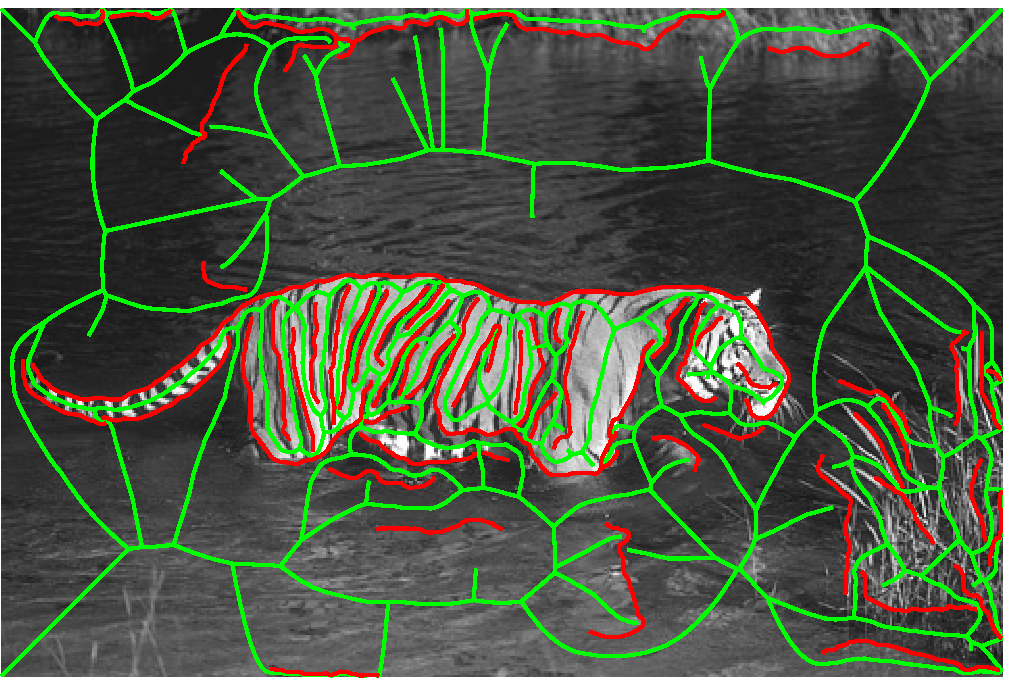
\includegraphics[width=0.31\textwidth]{figs/tiger_lg_fig1.pdf}
{\footnotesize\textit{\textcolor{black}{b)}}}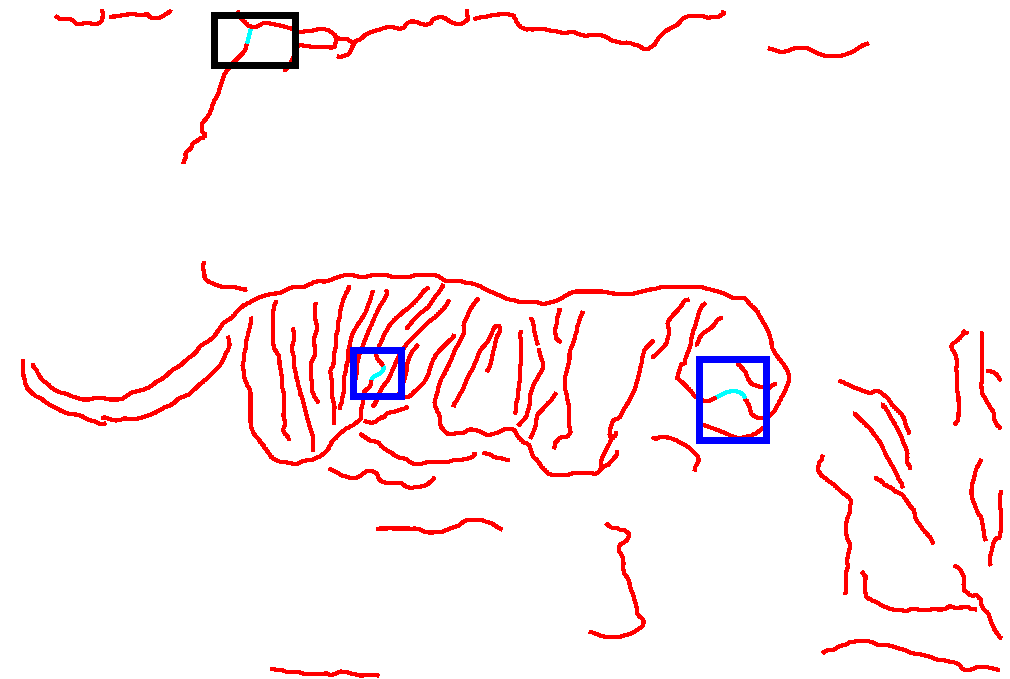
\includegraphics[width=0.31\textwidth]{figs/tiger_lg_fig2.pdf}
{\footnotesize\textit{\textcolor{black}{c)}}}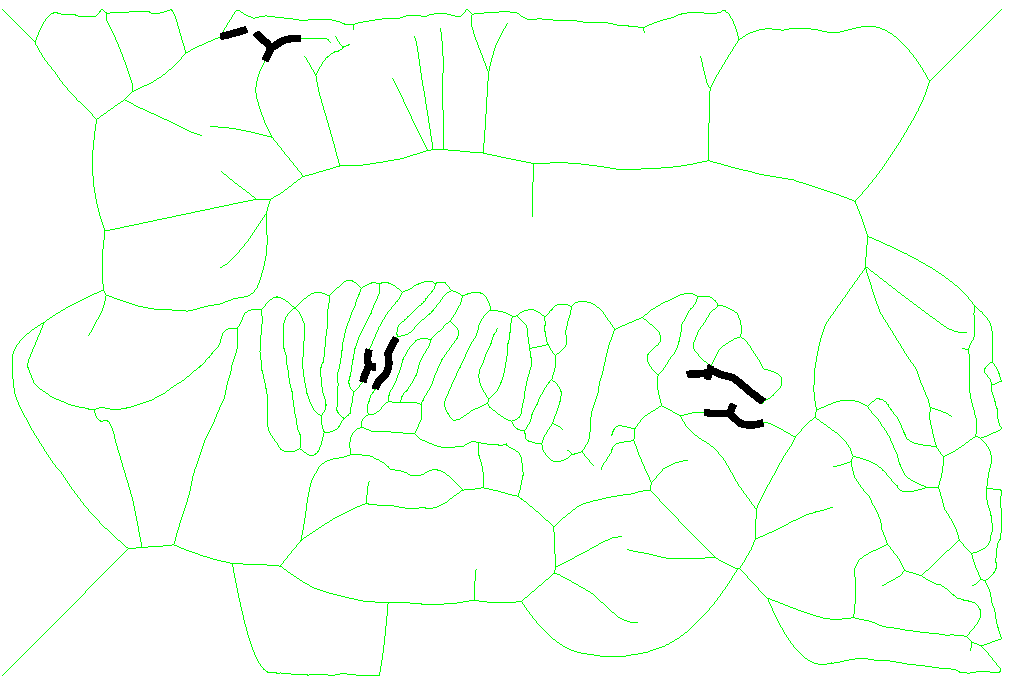
\includegraphics[width=0.31\textwidth]{figs/tiger_lg_fig3.pdf}
\caption{A naive implementation of inserting contours consists of taking the initial representation, a), and augmenting the contour set, sub-figure b), with new gap completions highlighted in \textcolor{cyan}{cyan} surrounded by black or \textcolor{blue}{blue} boxes indicating transversal or tangential completion respectively. If we recompute the shock graph based on this new augmented set, we notice that the number of new {\bf edges/nodes} compared to sub-figure a) is confined to a very small neighborhood of the overall graph. } 
\label{fig:lcs_motivate}
\end{figure*}

Local shock computation encompasses two operations: a set operation to update the contour set and a graph operation to re-compute the shock graph. While the former is trivial the latter is much more involved. Given a shock graph of $E$ directed shock links and $V$ vertices local shock computation is a graph operation where a subset of $E$ edges and $V$ vertices are deleted and replaced with a new set of edges and nodes. Intuitively local shock computation can be seen as the stitching of a new smaller shock graph into a larger whole. The first step of updating the shock graph is to identify and delete the subset (links and vertices) of the graph that will change if the underlying contour map is altered.  During shock computation the algorithm of~\cite{Tamrakar:Kimia:Shock} explicitly associates each contour element (point or line) with a time (distance) ordered list of shock links originating from that specific contour element. Similarly, each shock link is associated with the pair of contour elements  (point or line) that spawned it. If we are interested in deleting a contour approximated by a $T$ line segments then the union of all $T$ shock link lists identifies the shock segments that need to be removed. Given that each shock link represents a time-order event (creation of a shock node or link) its removal requires us to consider how that will affect past and future events. It is shown in~\cite{Tamrakar:Kimia:Shock}  that deleting a shock link requires us to delete all future child shock links until we reach the first node that is exclusively composed of neighboring parent shocks, Figure~\ref{fig:delete_shocks}\textcolor{red}{(a,b)}.  These “future” child shock links are not identified by the initial set of lists as they only capture the shock links forming the loop directly around the contour to be removed. The deletion process will recursively keep deleting elements until this condition is met. After all links are removed nodes lacking any child shocks are subsequently deleted, Figure~\ref{fig:delete_shocks}\textcolor{red}{(c)}. Figure~\ref{fig:loop_step}\textcolor{red}{(a,b)} shows a realistic example where the elements affected extend beyond the immediate loop encircling the orange contour to be removed.   


\begin{figure*}[!ht]
\centering
{\footnotesize\textit{\textcolor{black}{a)}}}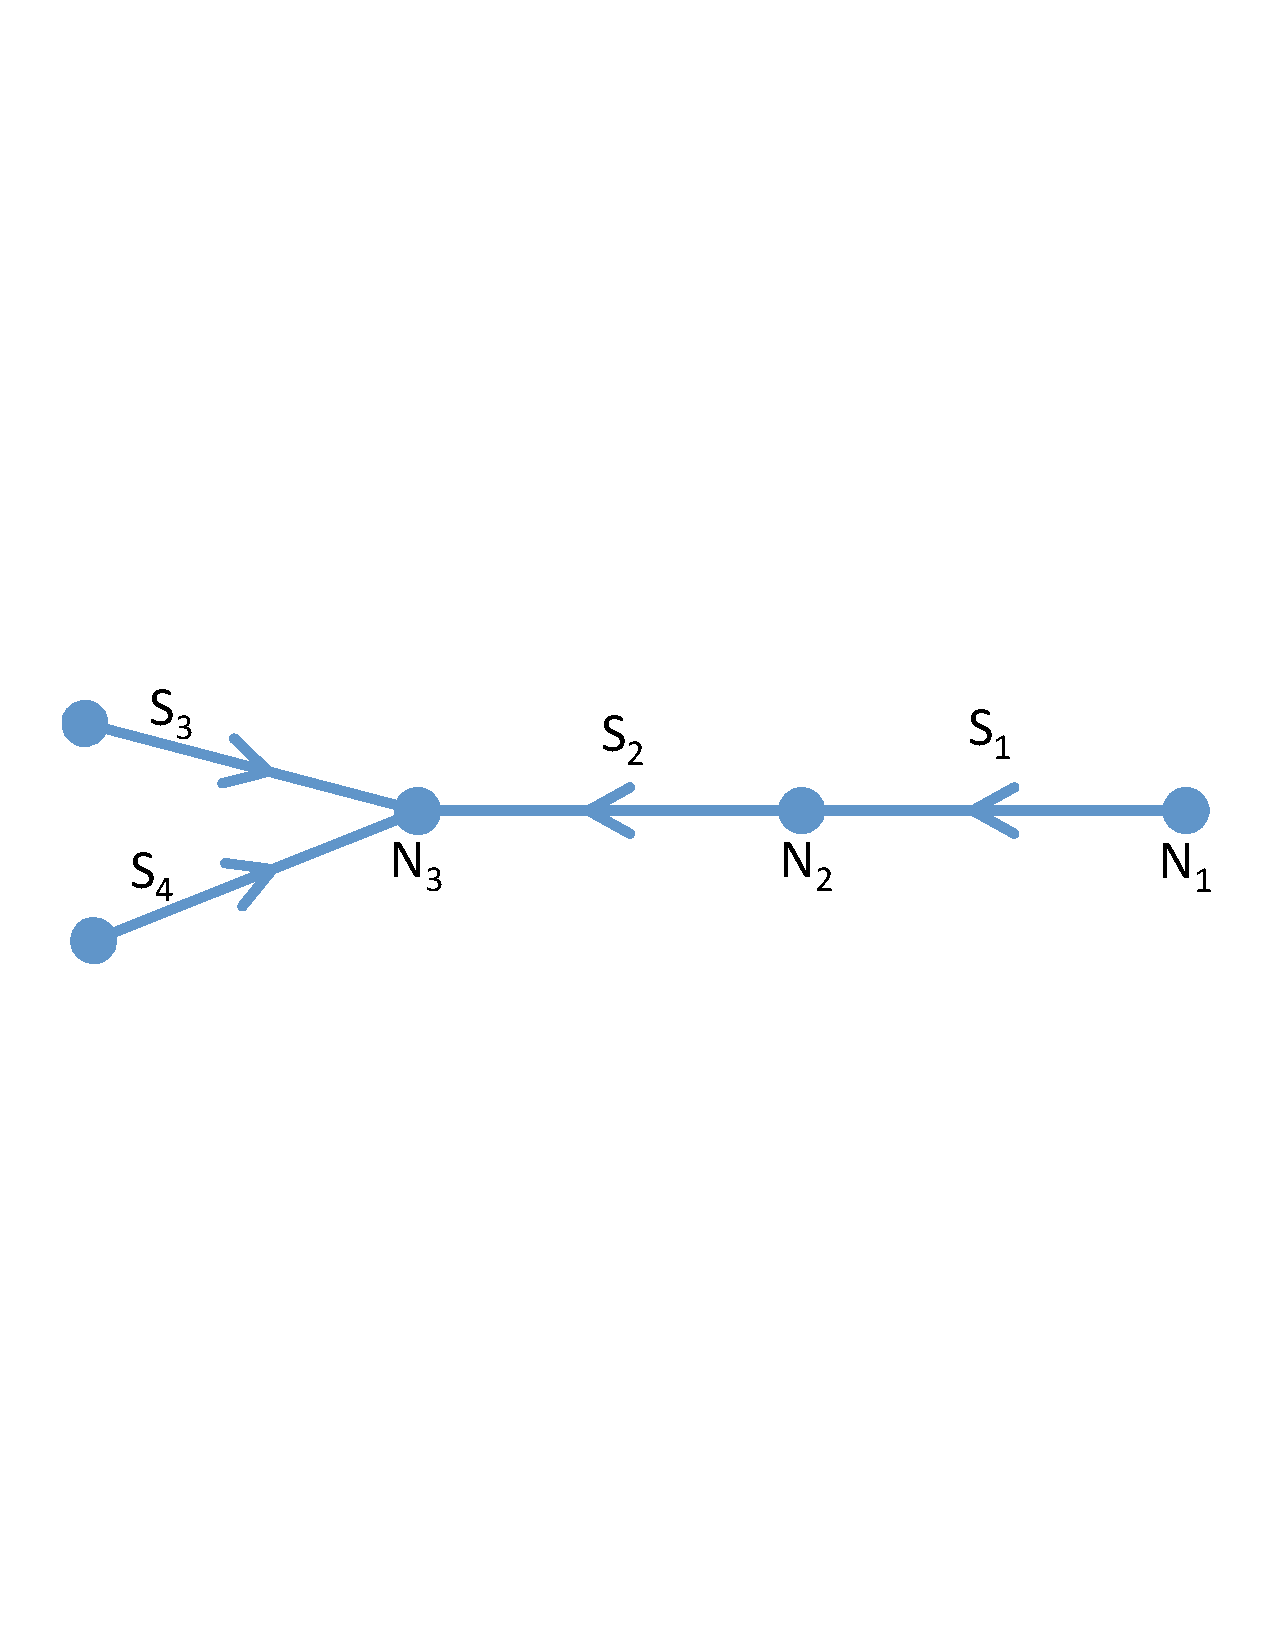
\includegraphics[width=0.33\textwidth]{figs/delete_shocks.pdf}
{\footnotesize\textit{\textcolor{black}{b)}}}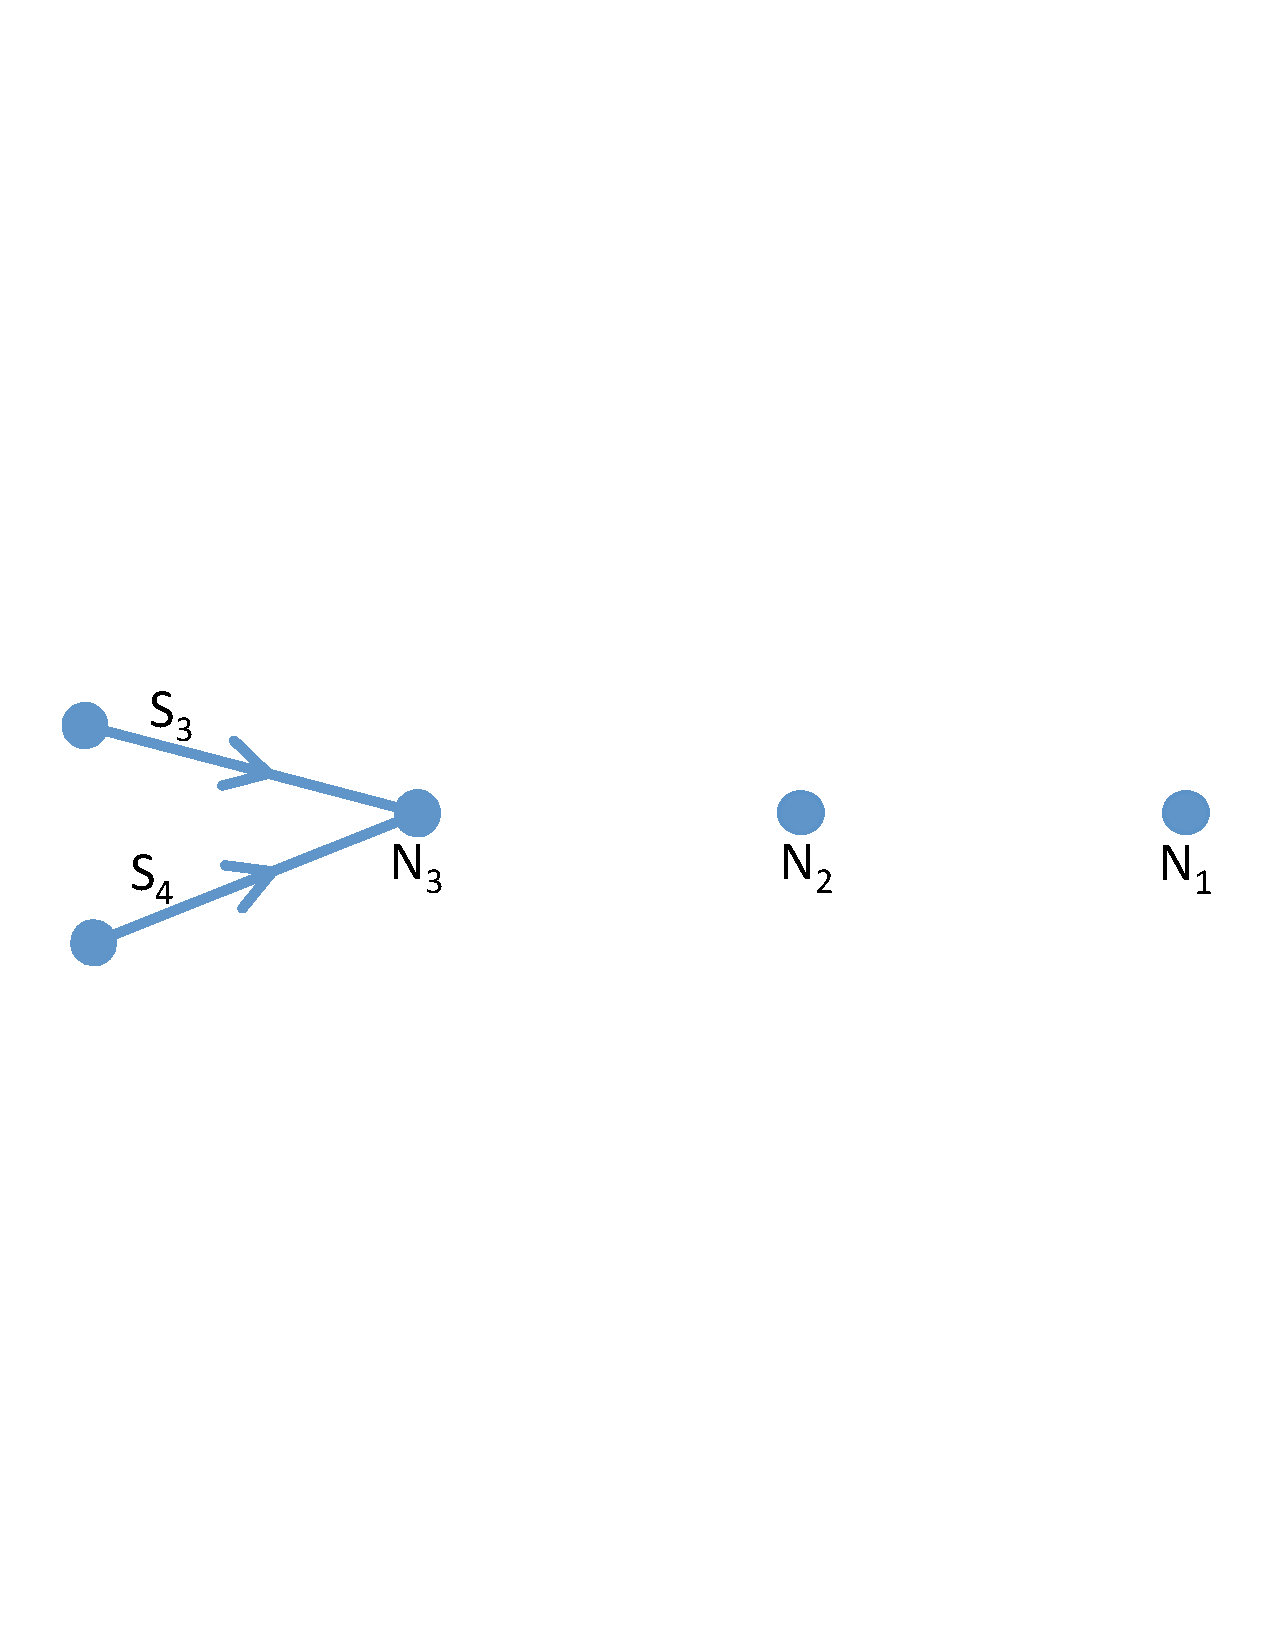
\includegraphics[width=0.33\textwidth]{figs/delete_shocks_2.pdf}
{\footnotesize\textit{\textcolor{black}{c)}}}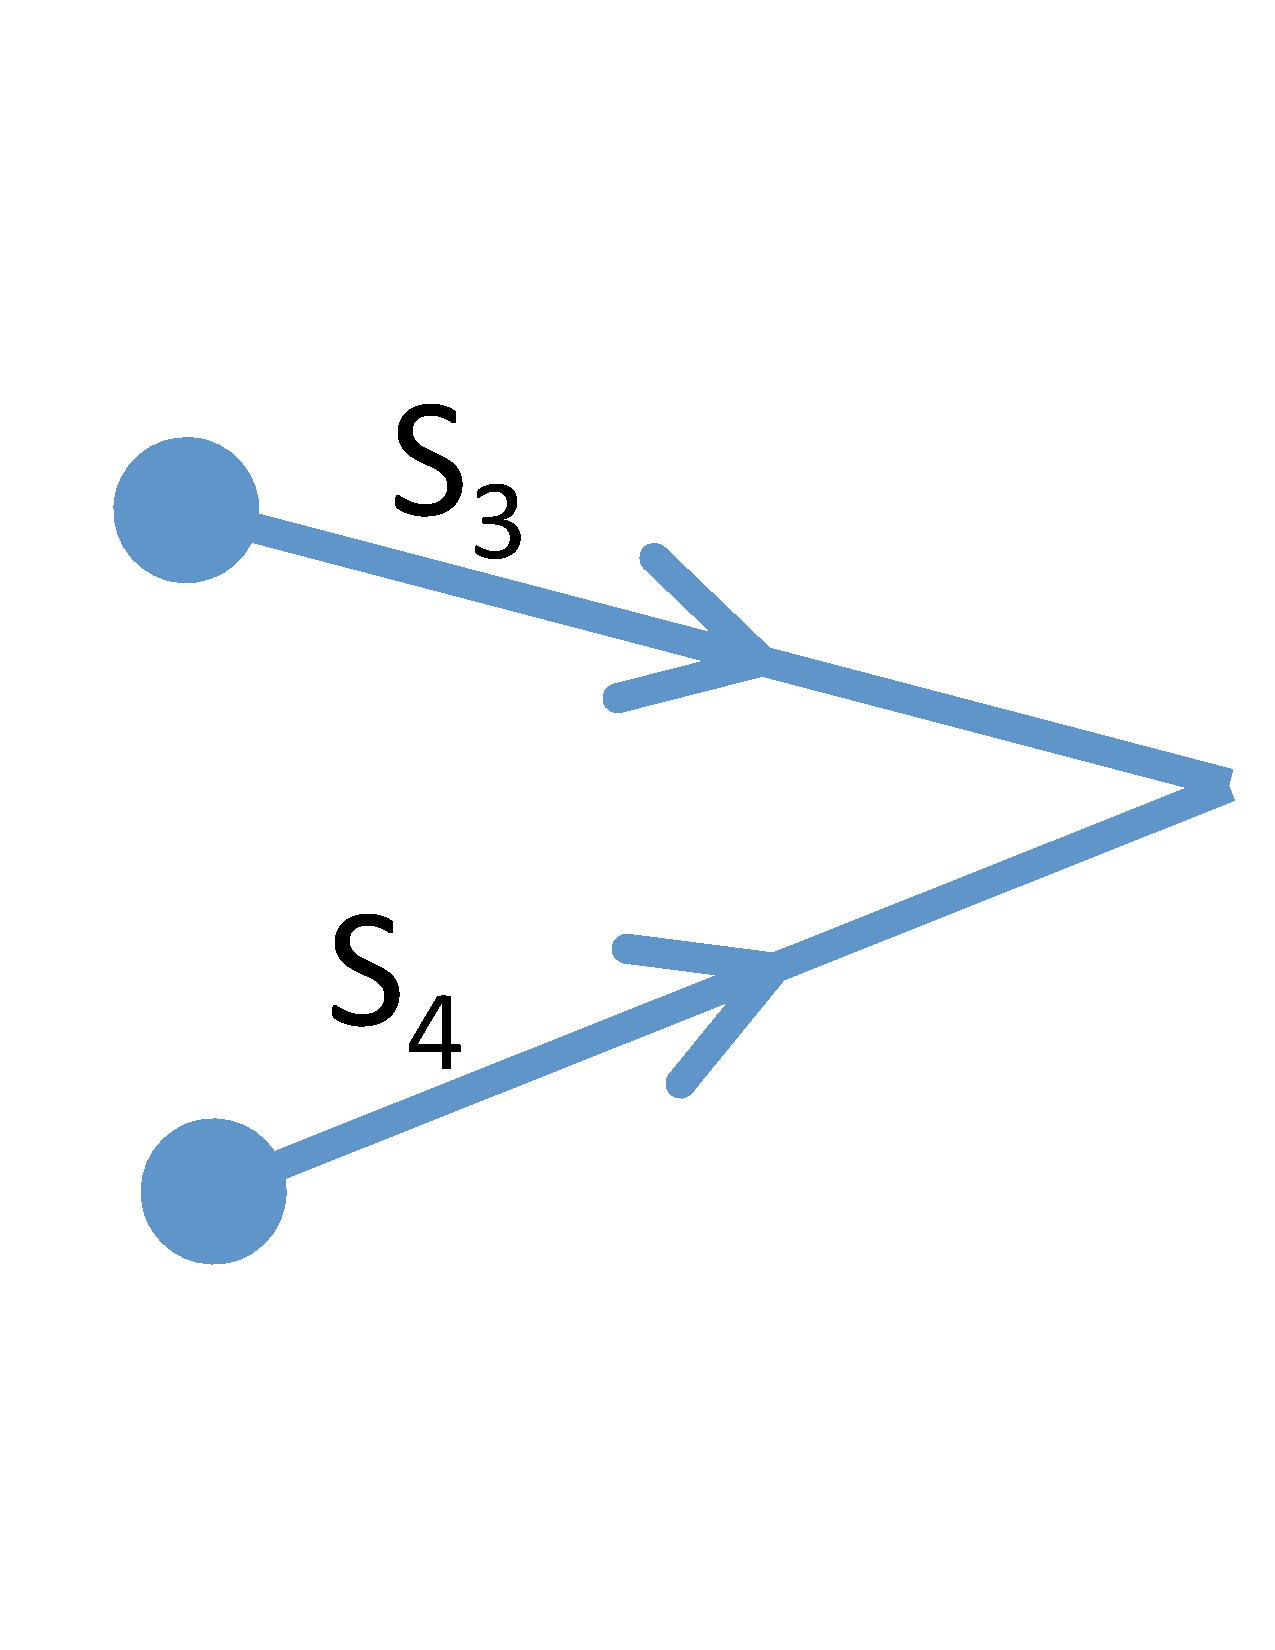
\includegraphics[width=0.12\textwidth]{figs/delete_shocks_3.pdf}
\caption{(a) A synthetic example of a shock graph where we consider the deletion of $S_1$. $S_1$ is a child shock of Node $N_1$. (b) Deleting $S_1$ requires us to delete all future child shocks. Given that $S_1$ is a parent shock of $N_2$ the child shock of $N_2$, $S_2$, cannot exist without the parent. This process stops at $N_3$ as the two parent shocks $S_3$ and $S_4$ have occurred before the creation of $S_1$ and as such are not affected. (c) The picture after removal of the Nodes $N_1$ and $N_2$. } 
\label{fig:delete_shocks}
\end{figure*}



\begin{figure*}[!ht]
\centering
{\footnotesize\textit{\textcolor{black}{a)}}}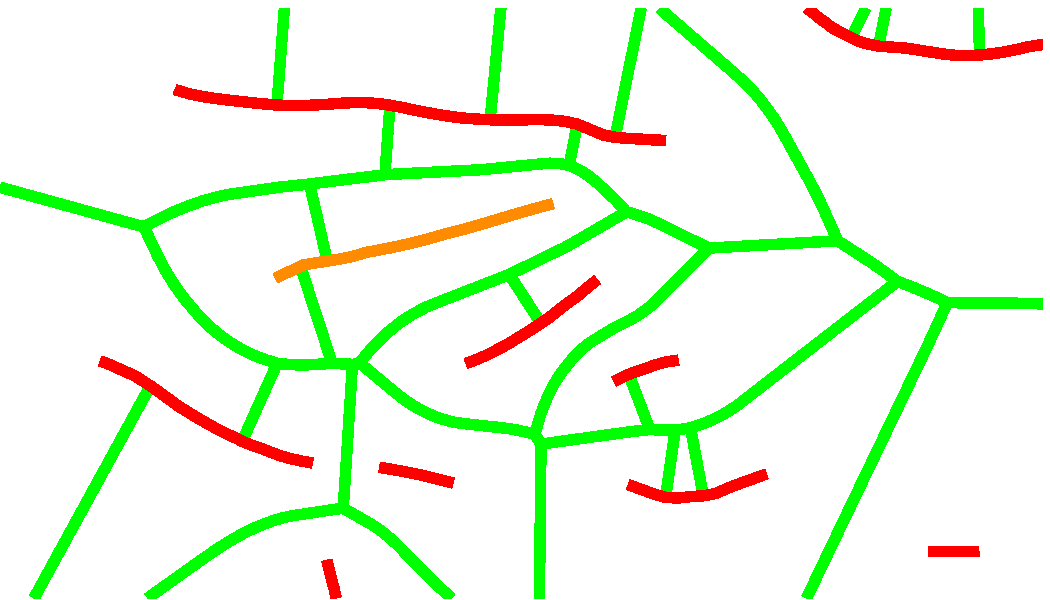
\includegraphics[width=0.31\textwidth]{figs/giraffe_before_shocks.pdf}
{\footnotesize\textit{\textcolor{black}{b)}}}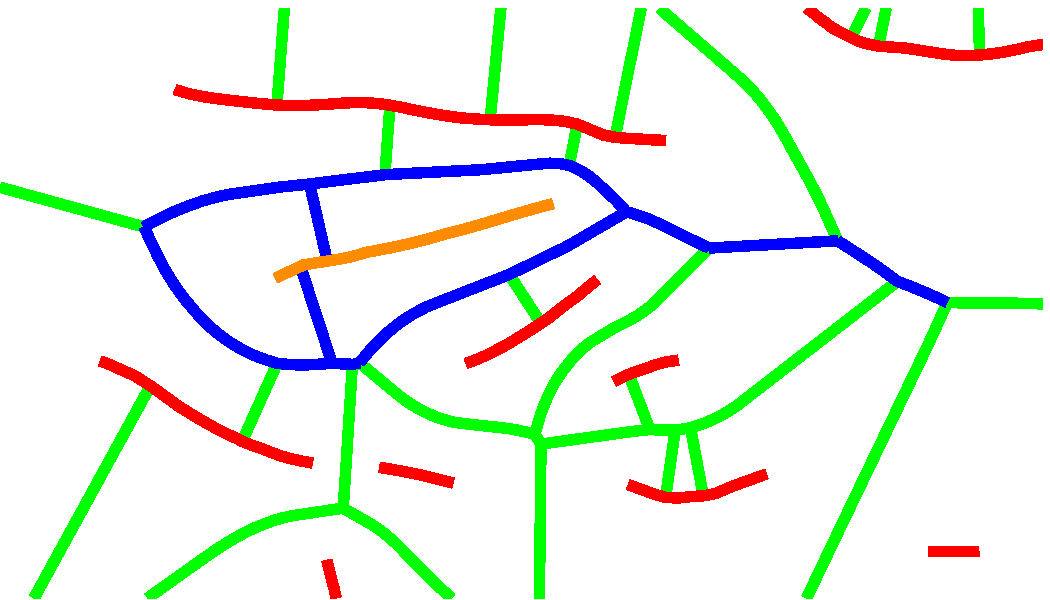
\includegraphics[width=0.31\textwidth]{figs/giraffe_before_shocks_identify.pdf}
{\footnotesize\textit{\textcolor{black}{c)}}}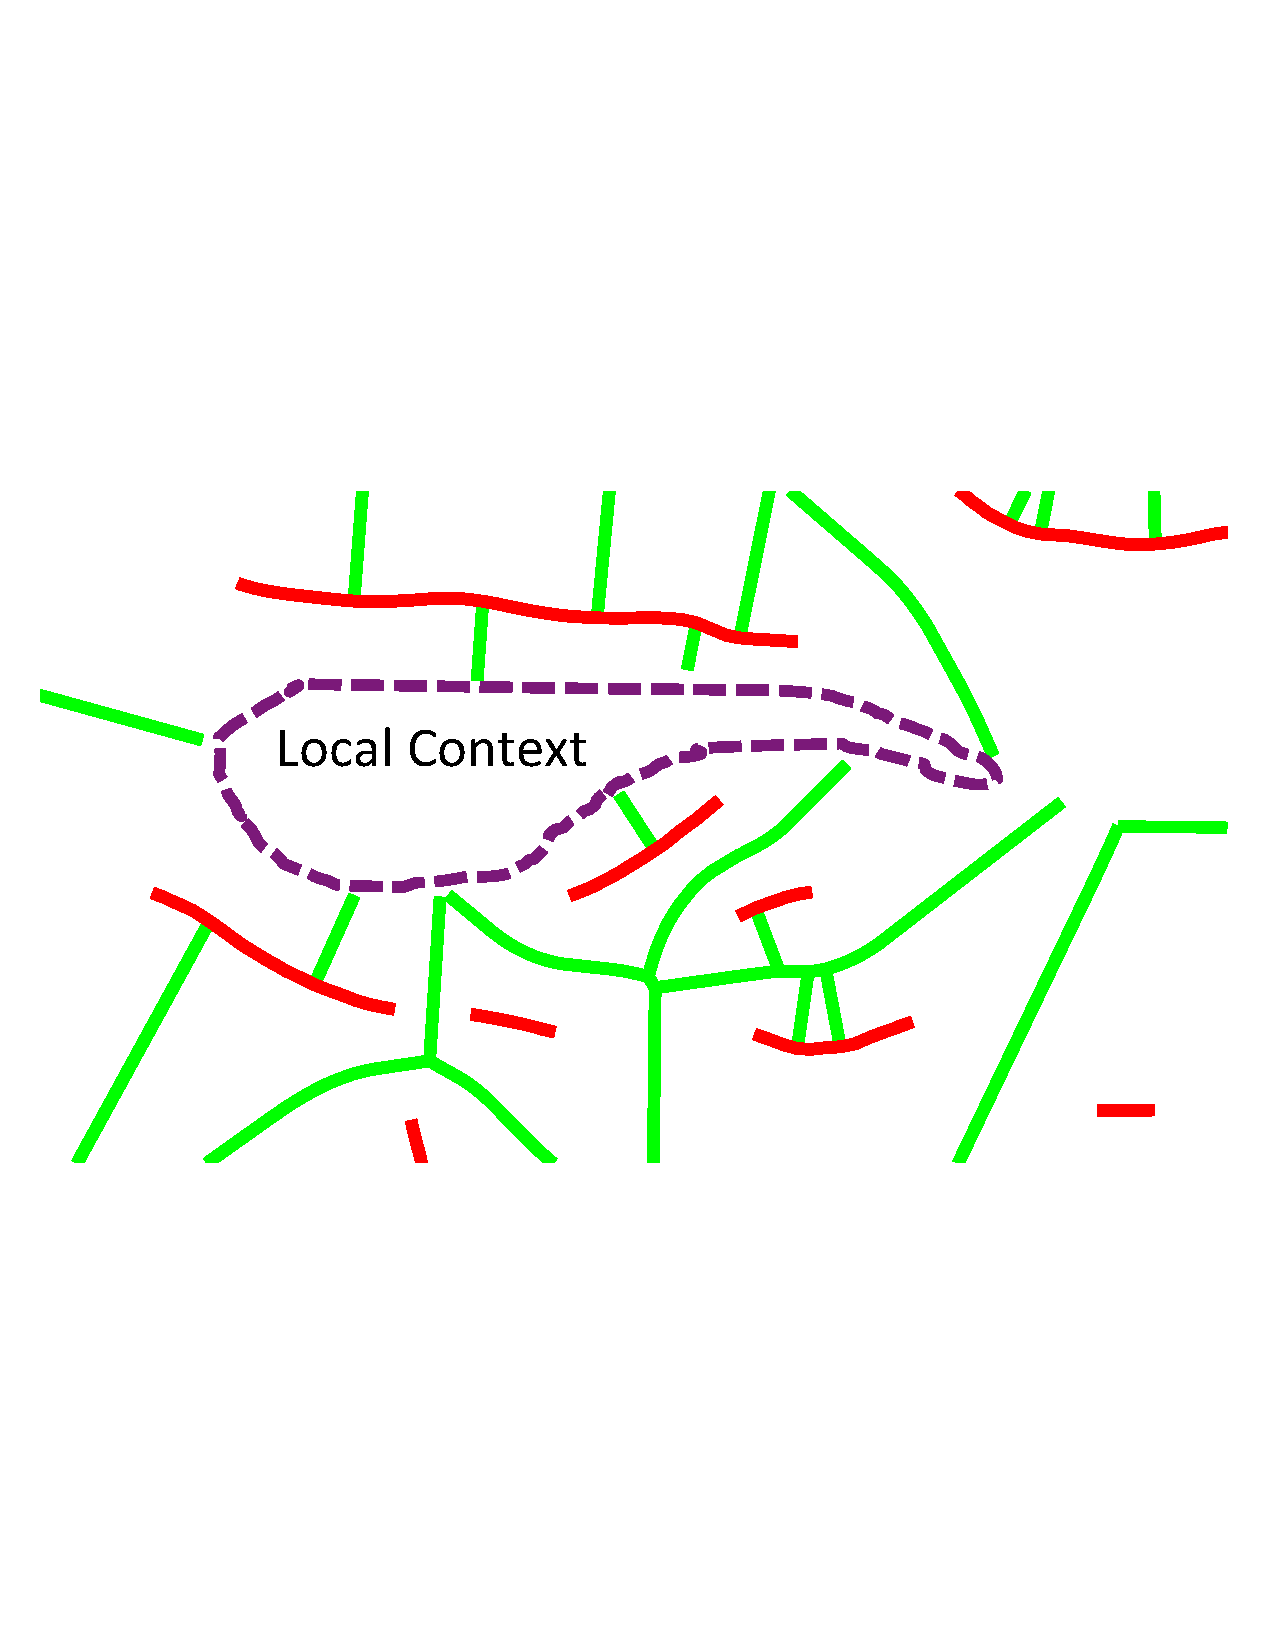
\includegraphics[width=0.31\textwidth]{figs/giraffe_remove_shocks_identify.pdf}
{\footnotesize\textit{\textcolor{black}{d)}}}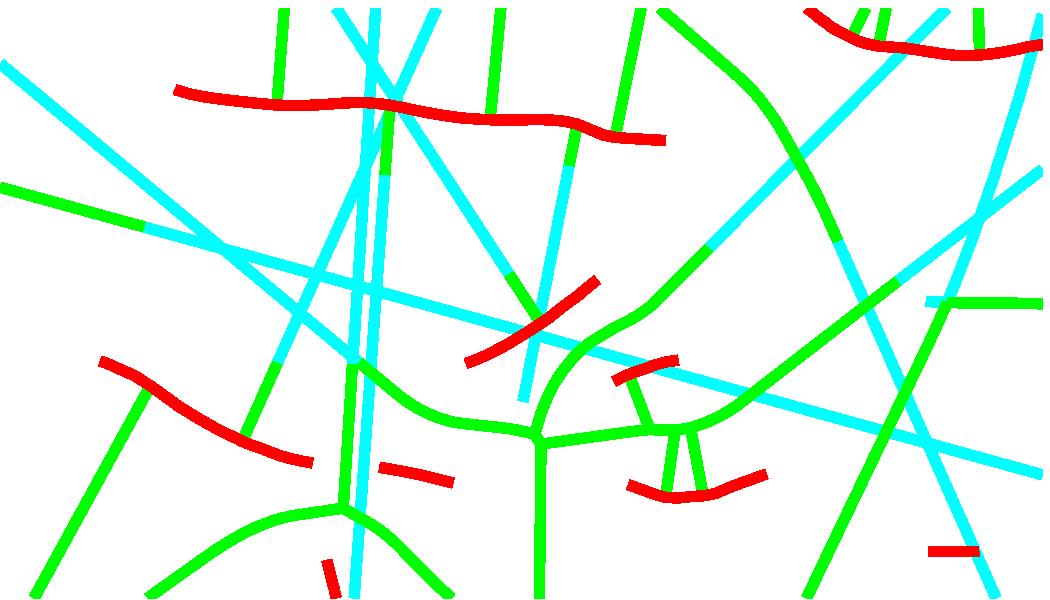
\includegraphics[width=0.31\textwidth]{figs/giraffe_reactive_shocks.pdf}
{\footnotesize\textit{\textcolor{black}{e)}}}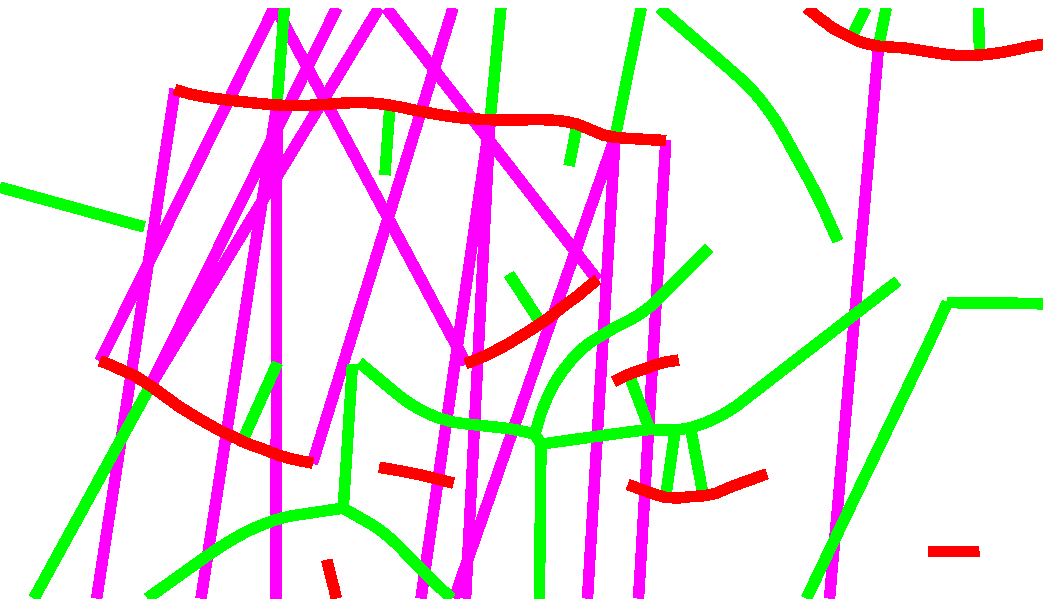
\includegraphics[width=0.31\textwidth]{figs/giraffe_reactive_shocks_contact.pdf}
{\footnotesize\textit{\textcolor{black}{f)}}}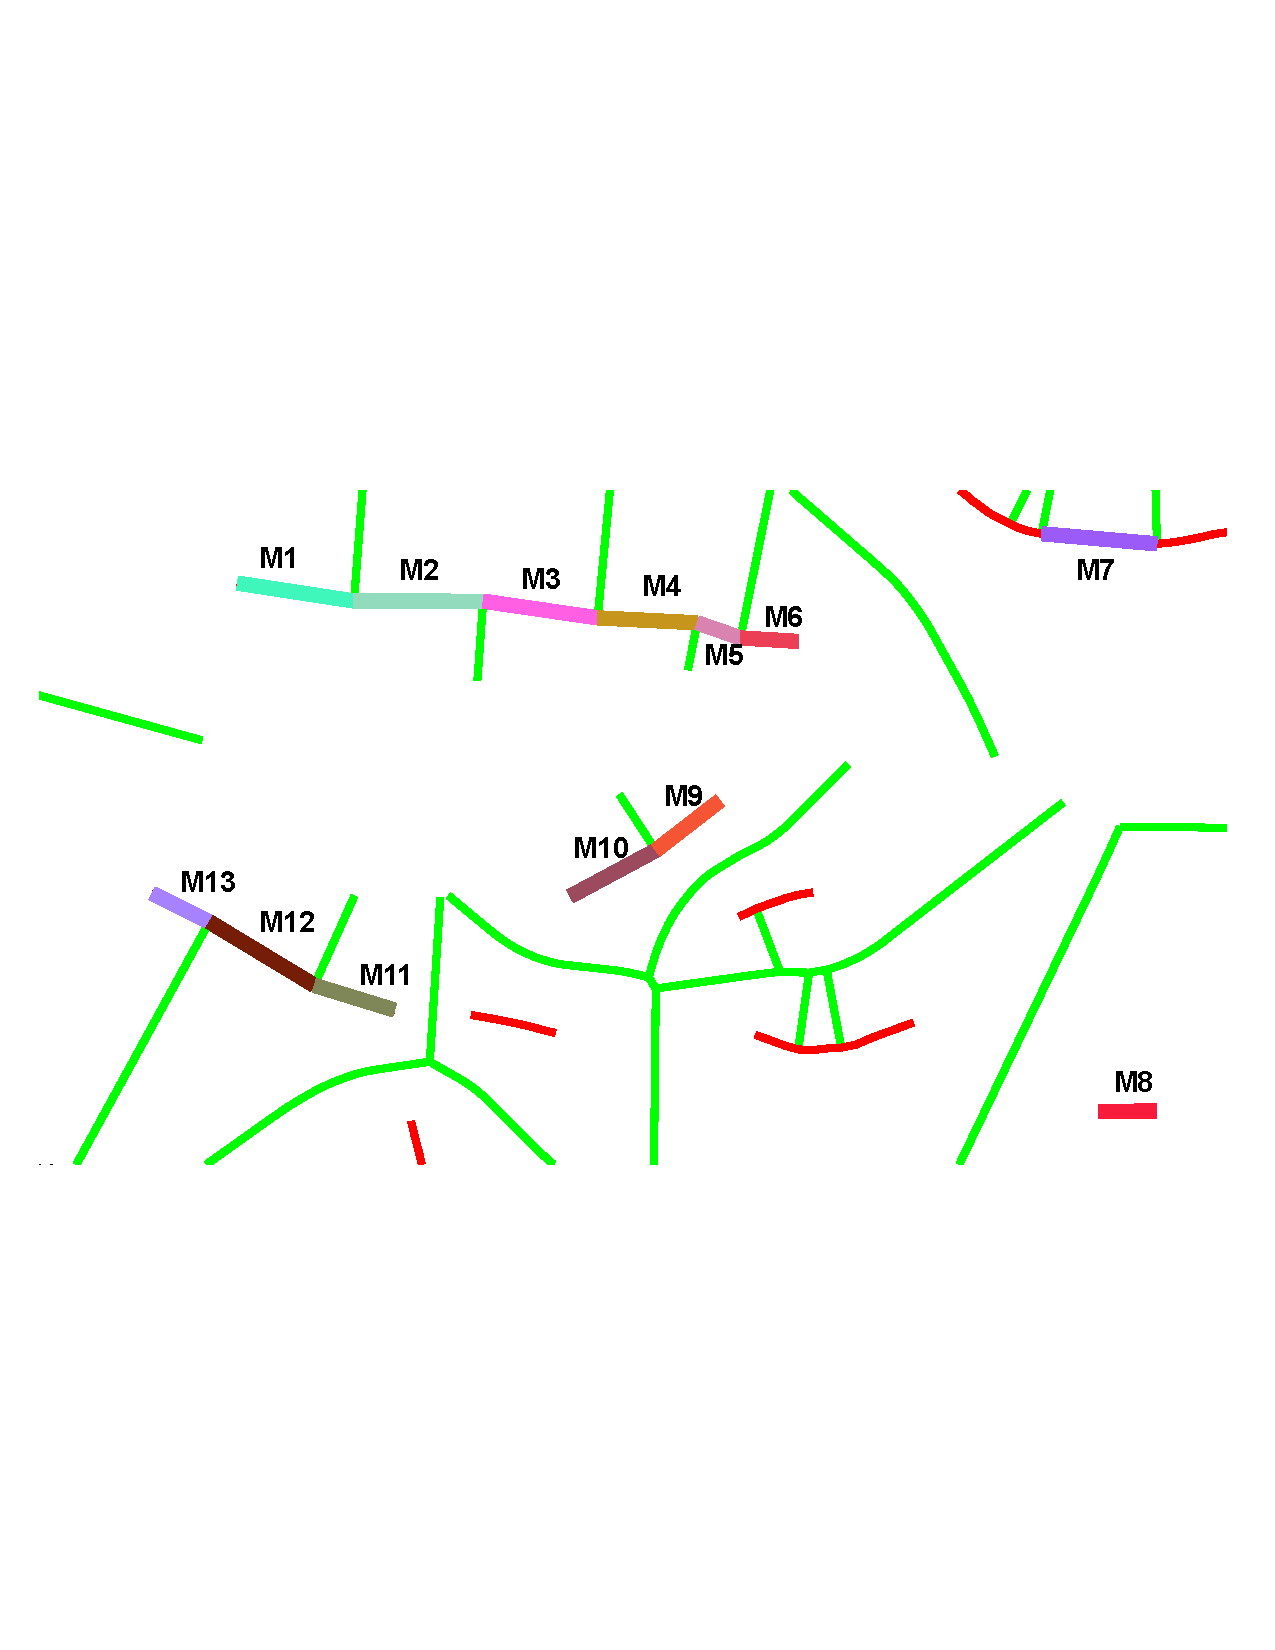
\includegraphics[width=0.31\textwidth]{figs/giraffe_reactive_M_contours.pdf}
{\footnotesize\textit{\textcolor{black}{g)}}}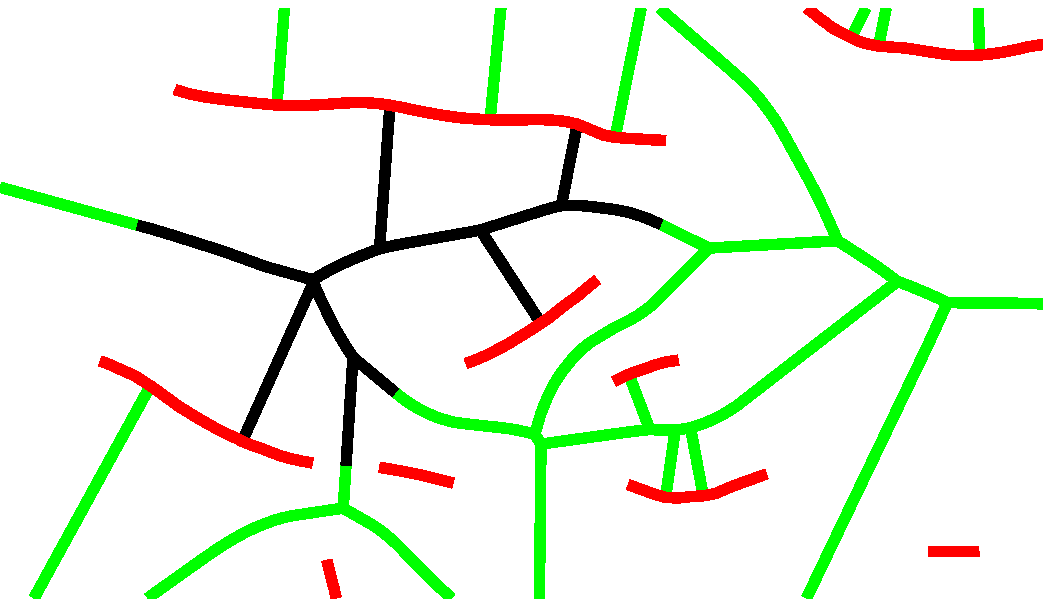
\includegraphics[width=0.31\textwidth]{figs/giraffe_after_shocks.pdf}

\caption{a) A local area of the shock graph where we consider the removal of the contour highlighted in orange. b) We highlight in blue the shock links that are affected by removal of this contour. c) We proceed to remove these elements leaving an area which has roughly been outlined called the local context. d) We reactivate all shocks impinging on this area in cyan. e) We reactive ``contact'' shocks impinging on this area in magenta. f) We determine the subset $M$ of contour elements involved with each element labeled $M_1$ to $M_13$. The interaction of these boundary elements lead to a set of $M^2$ candidate shock sources. f) The final picture after rerunning Lagrangian propagation give the ``active'' and candidate sources. } 
\label{fig:loop_step}
\end{figure*}

If one considers the union of influence zones associated with each deleted shock link this defines a local area, ``local context'', over which new shocks need to be inserted, Figure~\ref{fig:loop_step}\textcolor{red}{(c)}. The next step is to determine the set of new shock links and nodes that need to be inserted into the graph confined to this area. This step requires us to consider existing shock links impinging on the local context and the creation of totally new shock links determined by the interaction of contour elements defining the local context. Impinging waves are simply reactivated by resetting the end time of that specific shock link to infinity, which we refer to as “active” shocks, highlighted in cyan in Figure~\ref{fig:loop_step}\textcolor{red}{(d)}. Along with these active shocks we must reactivate the ``contact'' shocks~\cite{Tamrakar:Kimia:Shock} also impinging on the local context. To determine the new shock links and nodes we consider the interaction of contour elements ($M$) associated with the previous deleted shock links, randomly colored in Figure~\ref{fig:loop_step}\textcolor{red}{(f)}. This subset of contour elements is then used to generate $M^2$ candidate sources identical to the initial stage of Lagrangian shock computation described in~\cite{Tamrakar:Kimia:Shock}. The set of “active” shocks (union of cyan and magenta in Figure~\ref{fig:loop_step}\textcolor{red}{(c,d)}) are inserted into one-time ordered list and the $M^2$ candidate sources are inserted into another. At this point we simply rerun the propagation step of Lagrangian shock computation utilizing these two lists to determine the valid portion of these shock bisectors and update the shock graph accordingly, Figure~\ref{fig:loop_step}\textcolor{red}{(g)}. The complexity of the local shock computation algorithm is equivalent to the overall global shock computation complexity of $N^2log(N)$ where $N$ is the number of interacting contours. However, in the case of local shock computation the number of interacting contours $M$ is order of magnitudes smaller than $N$.
 
A future improvement can be made is to reduce the quadratic dependence of our algorithm. In both the global and local case the runtime is dominated by the quadratic term ($M^2$ or $N^2$). Observe that even though the shock graph changes with the addition of new links and nodes with varying flows the local boundary elements $M$ are unchanged and furthermore are a subset of $N$. We can use this property to index the full $N^2$ contour elements and at run-time we can index each of the $M^2$ candidate sources. This provides a huge time improvement to now just $log(M)$ where we assume indexing a table has $O(1)$ time. 
	
The previous discussion centered on the steps to delete a contour. The insertion of a contour is identical to deleting a contour buy there are key differences. One restriction on this operation is that the insertion of a contour is constrained to interact with existing contour elements. Currently the algorithm only supports the case of inserting a contour between two endpoints of a contour or an endpoint and a contour. A random insertion of a contour into an arbitrary image location is not supported.  The key difference between inserting and removing a contour is the determination of which shock links/nodes are affected and need to be subsequently removed. If we consider the case of inserting a contour between two endpoints the shocks that are affected and subsequently the $M$ contour elements involved are found by simply traversing the shock list associated with each endpoint. However, once we insert a contour approximated by $Q$ polyline segments it is possible that these $Q$ polyline segments will affect more shock links/nodes than we initially deleted. The extra set of shock links/nodes affected is unknown initially but once we start the algorithm we can keep track of those shock links that are valid~\cite{Tamrakar:Kimia:Shock} and reincorporate them into our process. Initially the process begins by inserting $(M+Q)^2$ contour elements into the candidate source lists and the active shocks list is populated by our initial estimate of impinging shocks. After a single iteration of the algorithm it records whether any new shock/links nodes are affected. If that is the case then those shock links are subsequently deleted, and new sources are initiated from the boundary elements associated with these new deleted elements. Lagrangian shock computation is now rerun with this updated list of sources to consider. This process continues until the shock graph is valid as defined by ~\cite{Tamrakar:Kimia:Shock}. In practice at each single iteration the number of new contour element and shock elements increases by 3-5 from our initial estimate. Furthermore in many cases our initial estimate is sufficient and no extra iterations are needed. The complexity of the insertion case is $(Q+M)^2log(Q+M)$ where $Q+M$ reflects the total number of contours. The future improvement we outlined earlier only marginally helps here as it does capture the interaction of $Q$ with $M$ or $Q$ with itself.  Finally, just as important as complexity is correctness. After running this algorithm for either insertion or deletion we check whether the resulting entire shock graph is valid as defined by ~\cite{Tamrakar:Kimia:Shock}. This ensures correctness of the graph for further downstream processing. 


\end{appendices}
